\chapter{Development of a New Digital Data Acquisition System}
\label{ch:DAQ}

%%%%%%%%%%%%%%%%%%%%%%%%%%%%%%%%%%%%%%%%%%%%%%%%%%%%%%%%%%%%%%%%%%%%%%%%%%%%%%%

\section{Introduction}

A new digital data acquisition system (DAQ) has been developed for use with the focal-plane detector package \cite{Marshall2019} and Enge Split-Pole Spectrograph at the Triangle Universities Nuclear Laboratory (TUNL). A new digitizer will replace the traditional analog modules and analog-to-digital converter (ADC) that have been used for the focal-plane detector electronics at TUNL. This chapter serves to highlight the components of the upgraded system and my contributions to the development and testing of the DAQ, as well as a new GUI \texttt{EngeSpec}. The motivation for upgrading to a digital DAQ will be provided in Section \ref{sec:motivation}. An overview of the CAEN V1730 digitizer will be given in Section \ref{sec:digitizer}. The custom frontend DAQ software will be presented in Section \ref{sec:frontend}. %The custom GUI \texttt{EngeSpec} will be showcased in Section \ref{sec:EngeSpec}. 
Finally, Section \ref{sec:DAQ_Tests} will highlight energy and timing resolution tests of the digital DAQ with $^{152}$Eu and $^{60}$Co radiation data using the \texttt{EngeSpec} GUI and its updated sort routine.

%system (DAQ) and graphical user interface (GUI)

%%%%%%%%%%%%%%%%%%%%%%%%%%%%%%%%%%%%%%%%%%%%%%%%%%%%%%%%%%%%%%%%%%%%%%%%%%%%%%%

%\pagebreak
\section{Background and Motivation} \label{sec:motivation}

% Note: "Analog DAQ" is probably not a thing. Instead, have this part be about Analog Modules vs. Digitizers. The "DAQ" should only refer to the custom DAQ software, i.e. the digitizer and its firmware are not part of the DAQ, nor is the EngeSpec GUI.

Nuclear physics experiments involving the detection of particles or $\gamma$-rays require a method of converting detected counts into numerical data. 
%The DAQ is responsible for collecting, processing, sorting, storing, and visualizing events from radiation detectors.
%\footnote{Some define the term DAQ as being associated with only the collection, sorting, and storing of data, while processing and visualizing are separate functions reserved for signal-processing modules and GUIs, respectively. Here, we define a DAQ system as the entire process of acquiring data.}. 
Fig. \ref{fig:traditional_electronics} illustrates the components of the traditional data acquistion system (DAQ). Detectors first convert each particle or $\gamma$-ray event into an analog electrical signal, or pulse. Pulse processing then alters the detector signal so as to reduce noise and amplify the pulse to sufficient levels for extraction. At this point, the energy and timing of the event can be determined by further processing. This processing is traditionally performed by a network of analog modules, where the processed pulse is then converted to a digital pulse via an analog-to-digital converter (ADC). The digital pulse can finally be read by a computer and collected by a DAQ software. The stored data can be visualized by a graphical user interface (GUI), which also sorts all of the data based on the corresponding detectors and observables and can perform several functions, such as curve fitting and gating.

\begin{figure}[t]
\centering
\begin{tikzpicture}[scale=1.25, every node/.style={transform shape}]

\node at (-2.5,0) {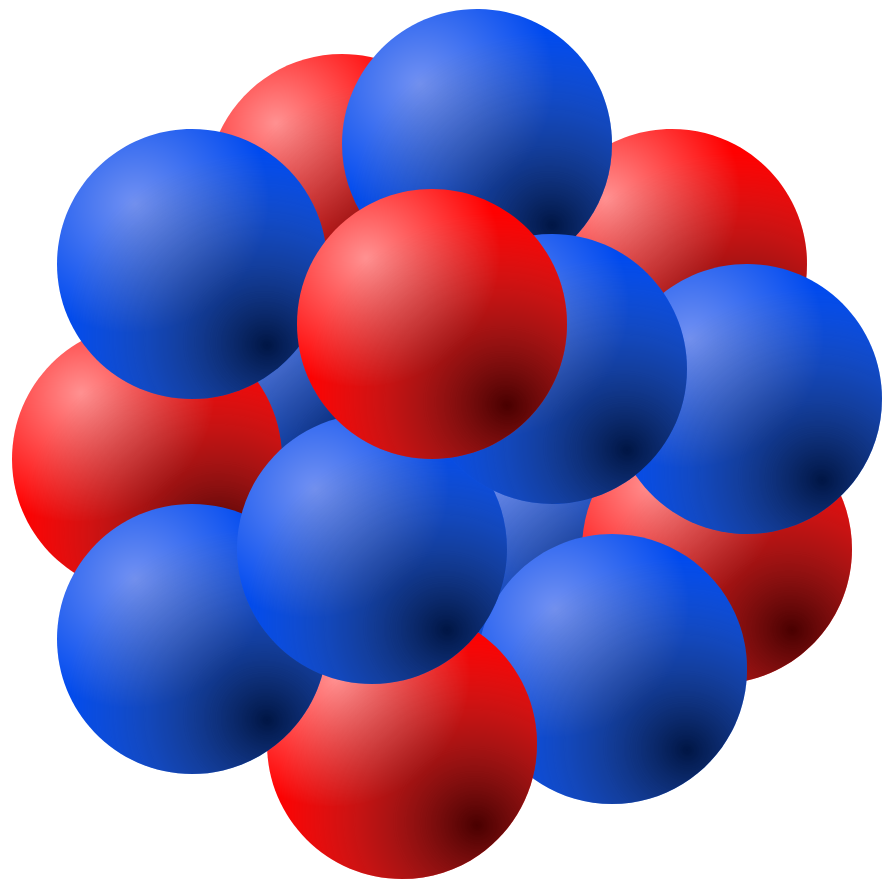
\includegraphics[scale=0.03]{Chapter-5/figs/nucleus.png}};
\node at (-2.5,-0.75) {\footnotesize{Particles}};
\draw[->] (-1.8,0) -- (-1.3,0);
\node[cylinder, draw, shape aspect=0.5, minimum height=0.5cm, scale=2,cylinder uses custom fill,cylinder body fill=gray!50,cylinder end fill=gray!25,rotate=180]{};
\begin{scope}[shift={(-0.6,0)}]
\node[cylinder, draw, shape aspect=0.5, minimum height=0.001cm, scale=1,cylinder uses custom fill,cylinder body fill=gray!50,cylinder end fill=gray!25,rotate=180]{};
\end{scope}
\node at (-0.2, -0.75) {\footnotesize{Detector(s)}};

%\node at (-0.25,-2.5) {\includegraphics[scale=0.08]{detector_signal}};
%\draw[->] (-0.2, -1.1) -- (-0.2, -1.6);
%\node at (-0.2, -3.5) {\footnotesize{Signal}};

\node at (1.05,-2.5) {\includegraphics[scale=0.08]{Chapter-5/figs/detector_signal.png}};
\draw[->] (1.05, -0.5) -- (1.05, -1.6);
\node at (1.05, -3.5) {\footnotesize{Signal}};

\draw[->] (0.8,0) -- (1.3,0);
\node at (2.7, -1.4) {\footnotesize{Analog Modules}};

\filldraw[fill=brown!70] (1.8,-1) rectangle (2.1,1);
\filldraw[fill=brown!70] (2.3,-1) rectangle (2.6,1);
\filldraw[fill=brown!70] (2.8,-1) rectangle (3.1,1);
\filldraw[fill=brown!70] (3.3,-1) rectangle (3.6,1);

\coordinate (A) at (1.45,-0.8,0);
\coordinate (B) at (1.95,0.8);
\coordinate (C) at (1.95,-0.8);
\coordinate (D) at (2.45,0.8);
\coordinate (E) at (2.45,-0.8);
\coordinate (F) at (2.95,0.8);
\coordinate (G) at (2.95,-0.8);
\coordinate (H) at (3.45,0.8);
\coordinate (I) at (3.45,-0.8);
\coordinate (J) at (3.95,0.8);

\filldraw[fill = white] (B) circle (0.5mm);
\filldraw[fill = white] (C) circle (0.5mm);
\filldraw[fill = white] (D) circle (0.5mm);
\filldraw[fill = white] (E) circle (0.5mm);
\filldraw[fill = white] (F) circle (0.5mm);
\filldraw[fill = white] (G) circle (0.5mm);
\filldraw[fill = white] (H) circle (0.5mm);
\filldraw[fill = white] (I) circle (0.5mm);

\draw (A) to [bend right = 10] (B);
\draw (C) to [bend right = 10] (D);
\draw (E) to [bend right = 10] (F);
\draw (G) to [bend right = 10] (H);
\draw (I) to [bend right = 10] (J);

\draw[->] (4.1,0) -- (4.6,0);
\filldraw[fill=black!50] (5,-1) rectangle (5.3,1);
\filldraw[fill = white] (5.15, 0.8) circle (0.5mm);
\filldraw[fill = white] (5.15, -0.8) circle (0.5mm);
\draw (4.65, -0.8) to [bend right = 10] (5.15, 0.8);
\draw (5.15, -0.8) to [bend right = 10] (5.65, 0.8);
\node at (5.15,-1.4) {\footnotesize{Analog}};
\node at (5.15,-1.75) {\footnotesize{to Digital}};
\node at (5.15,-2.05) {\footnotesize{Converter}};

\draw[->] (5.8,0) -- (6.3,0);
\node at (7.8,0) {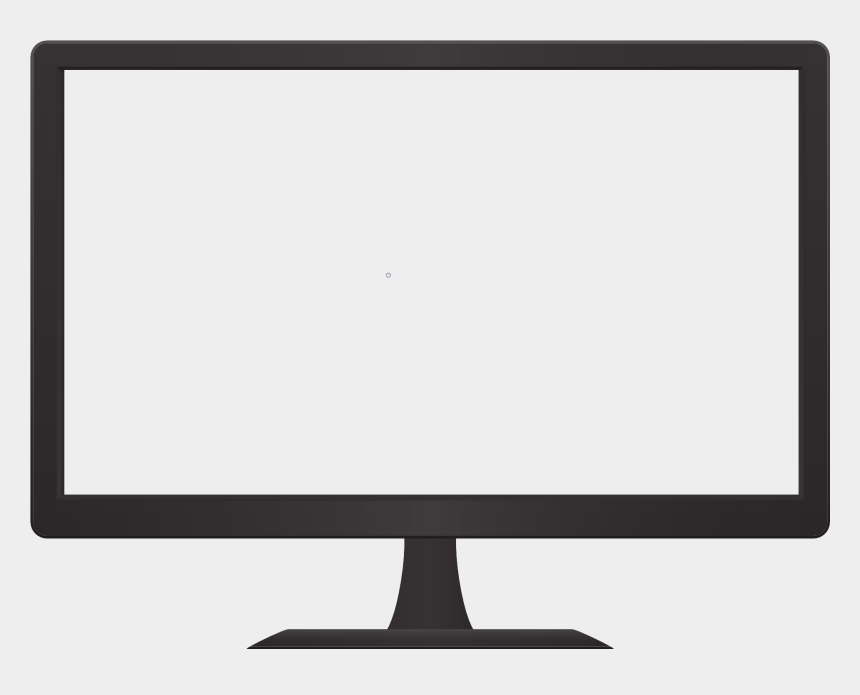
\includegraphics[scale=0.1]{Chapter-5/figs/computer_screen.png}};
\node at (7.8,-1.35) {\footnotesize{Computer / GUI /}};
\node at (7.8,-1.7) {\footnotesize{DAQ Software}};

\draw[->] (7.8, -1.9) -- (7.8, -2.4);
\node at (7.8,-3.4) {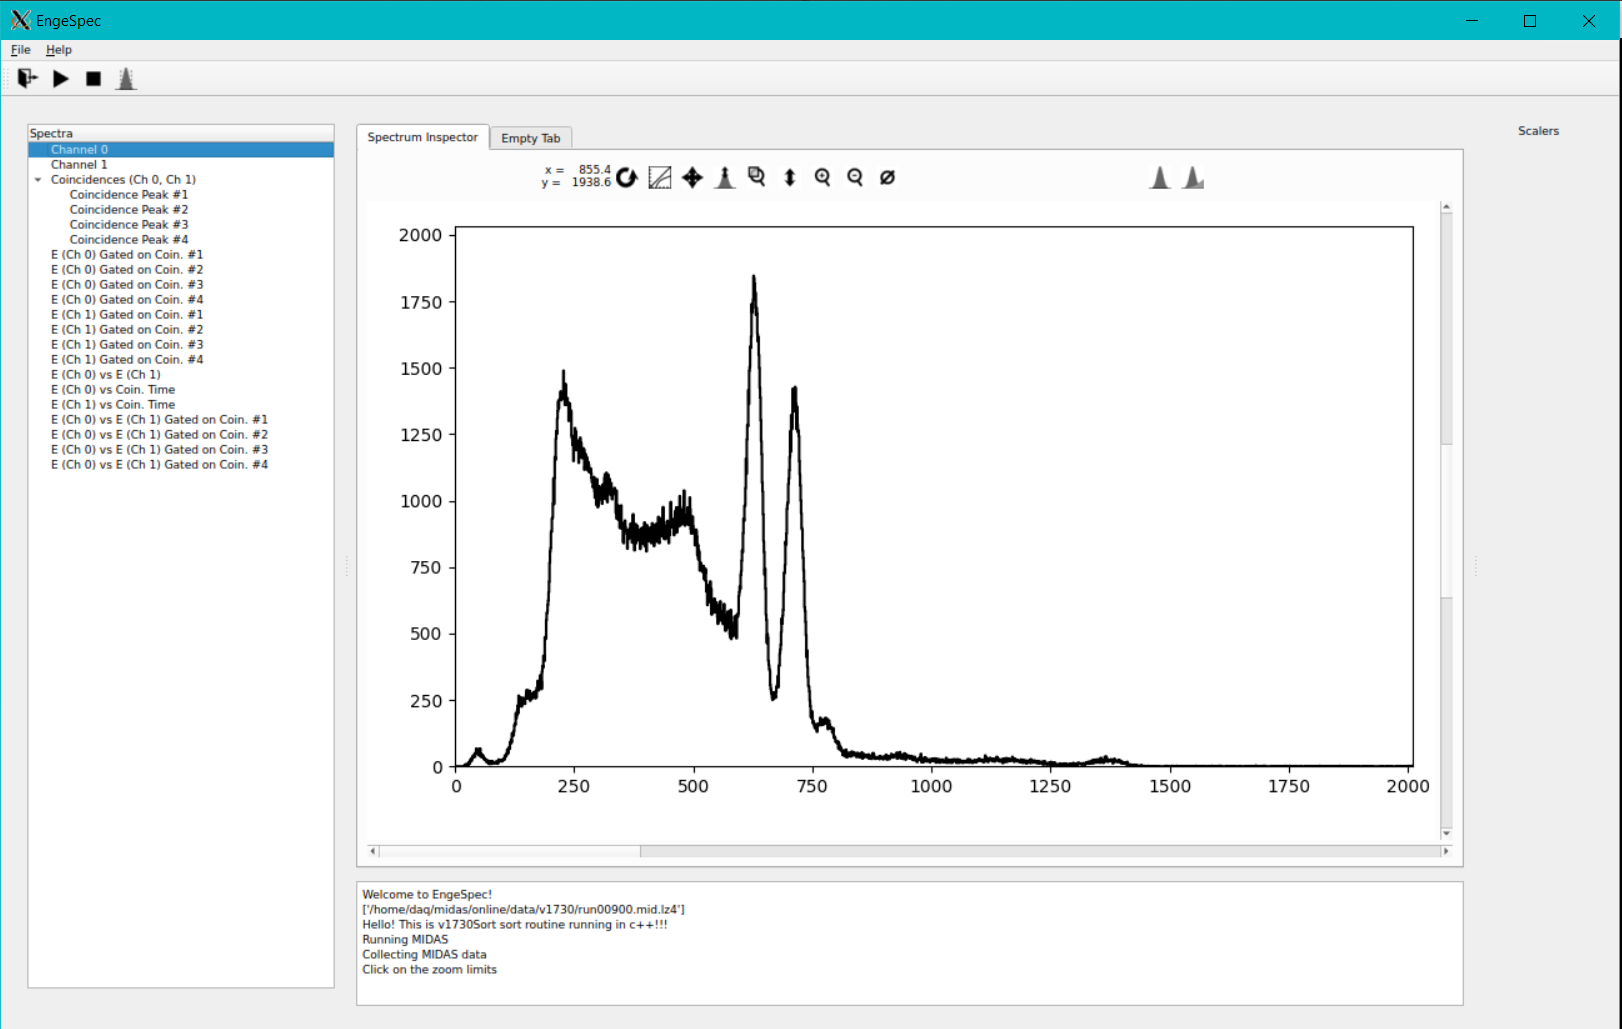
\includegraphics[scale=0.08]{Chapter-5/figs/Histogram_Co60.png}};
\node at (7.8,-4.5) {\footnotesize{Numerical Data}};

%\draw[decorate,decoration={brace,amplitude=5pt},rotate=270] (2.55,4.75) -- (2.55,3.25);
%\draw[decorate,decoration={brace,amplitude=5pt},rotate=270] (2.35,7.5) -- (2.35,3.25);
%\node at (4.3,-2.95) {Upgrading for};
%\node at (4.3,-3.25) {$^{87}\textnormal{Rb} + \gamma$ experiments};
%\draw[red] (2.5, -3.5) rectangle (6.1,-2.7);

\end{tikzpicture}
\caption{\label{fig:traditional_electronics}The traditional method of converting detected particles or $\gamma$-rays into numerical data using analog pulse-processing modules and an analog-to-digital converter (ADC).}
\end{figure}

The network of analog pulse-processing modules needed for nuclear physics experiments can be incredibly complex. Input and output cables connect modules together, and the vast number of cables can be cumbersome. Rearranging the network of modules between experiments amounts to physically altering the cable setup, which can lead to cable-mapping issues. The modules themselves also take up a significant amount of space. Hence, analog modules have an inherent portability problem.

A network of traditional analog modules can be replaced by a single digitizer, a module that performs the same pulse processing, but does so digitally after it samples the detector signals itself. Fig. \ref{fig:new_electronics} illustrates the new data acquisition method using a digitizer instead of analog modules and an ADC. Digitizers use firmware algorithms to emulate the functions of analog modules. Custom software is written by the user to perform specific functions that are needed for a given experiment. Changing the setup between experiments now amounts to altering existing code, rather than moving physical equipment. 

\begin{figure}[t]
\centering
\begin{tikzpicture}[scale=1.25, every node/.style={transform shape}]
\hspace{-0.6cm}

\hspace{1.6cm}
\node at (-2.5,0) {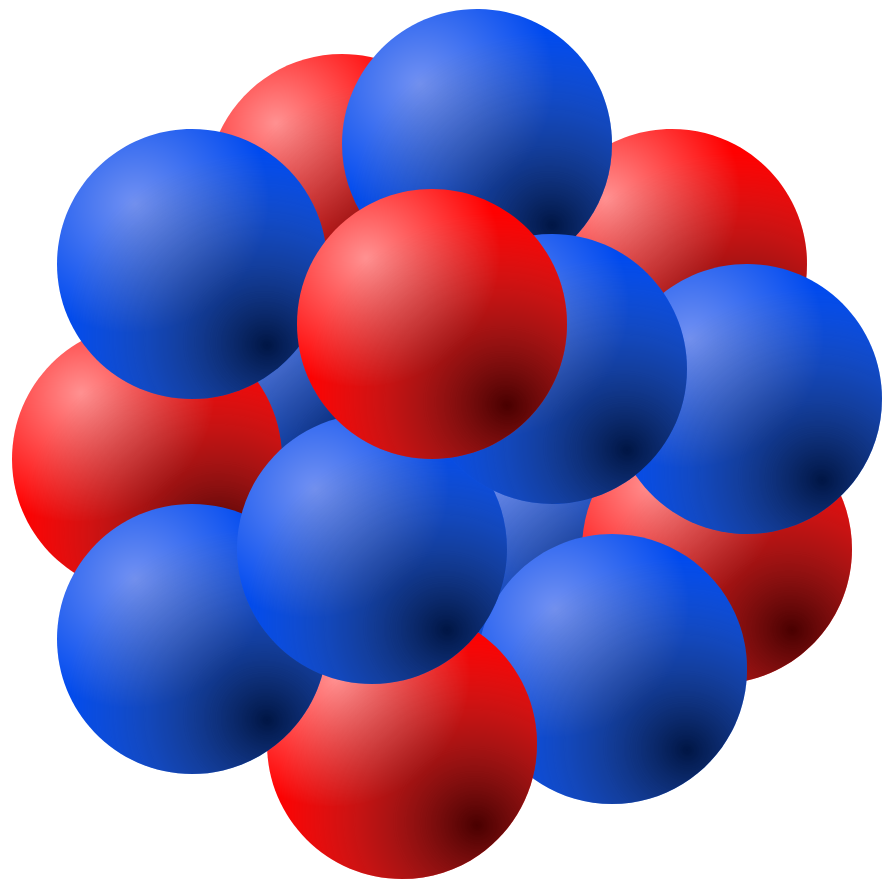
\includegraphics[scale=0.03]{Chapter-5/figs/nucleus.png}};
\node at (-2.5,-0.75) {\footnotesize{Particles}};
\draw[->] (-1.8,0) -- (-1.3,0);
\node[cylinder, draw, shape aspect=0.5, minimum height=0.5cm, scale=2,cylinder uses custom fill,cylinder body fill=gray!50,cylinder end fill=gray!25,rotate=180]{};
\begin{scope}[shift={(-0.6,0)}]
\node[cylinder, draw, shape aspect=0.5, minimum height=0.001cm, scale=1,cylinder uses custom fill,cylinder body fill=gray!50,cylinder end fill=gray!25,rotate=180]{};
\end{scope}
\node at (-0.2, -0.75) {\footnotesize{Detector(s)}};

\node at (1.05,-2.5) {\includegraphics[scale=0.08]{Chapter-5/figs/detector_signal.png}};
\draw[->] (1.05, -0.5) -- (1.05, -1.6);
\node at (1.05, -3.5) {\footnotesize{Signal}};

\draw[->] (0.8,0) -- (1.3,0);
%\node at (2.7, -1.4) {\footnotesize{Analog Modules}};
%\draw[->] (4.1,0) -- (4.6,0);

\hspace{-1.6cm}

\hspace{-1.6cm}
\filldraw[fill=red!50] (5,-1) rectangle (5.3,1);
\filldraw[fill = white] (5.15, 0.8) circle (0.5mm);
\filldraw[fill = white] (5.15, -0.8) circle (0.5mm);
\draw (4.65, -0.8) to [bend right = 10] (5.15, 0.8);
\draw (5.15, -0.8) to [bend right = 10] (5.65, 0.8);
\node at (5.15,-1.4) {\footnotesize{Digitizer}};
\hspace{1.6cm}

\hspace{-1.6cm}
\draw[->] (5.8,0) -- (6.3,0);
\node at (7.8,0) {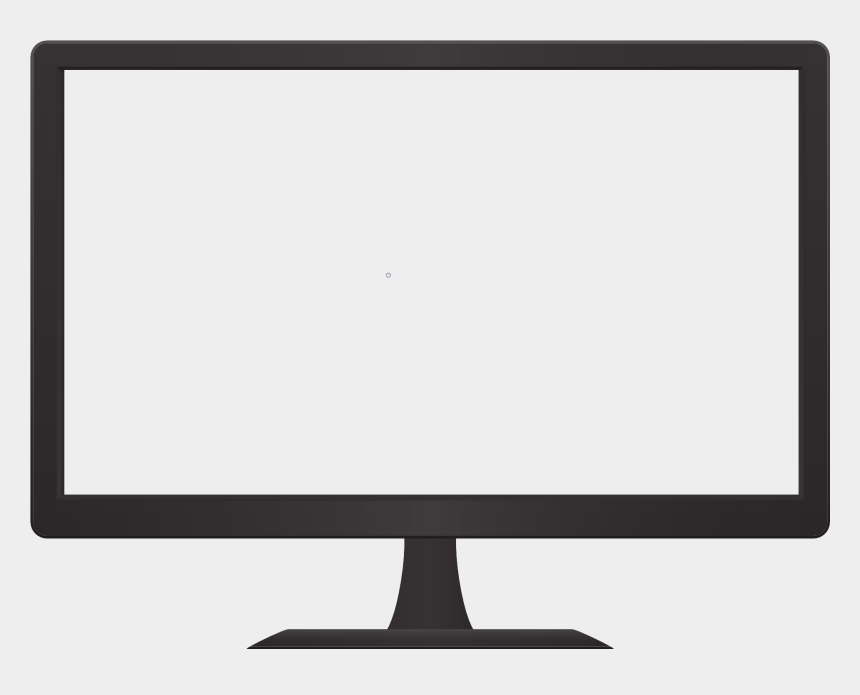
\includegraphics[scale=0.1]{Chapter-5/figs/computer_screen.png}};
\node at (7.8,-1.35) {\footnotesize{Computer / GUI /}};
\node at (7.8,-1.7) {\footnotesize{Custom DAQ Software}};

\draw[->] (7.8, -1.9) -- (7.8, -2.4);
\node at (7.8,-3.4) {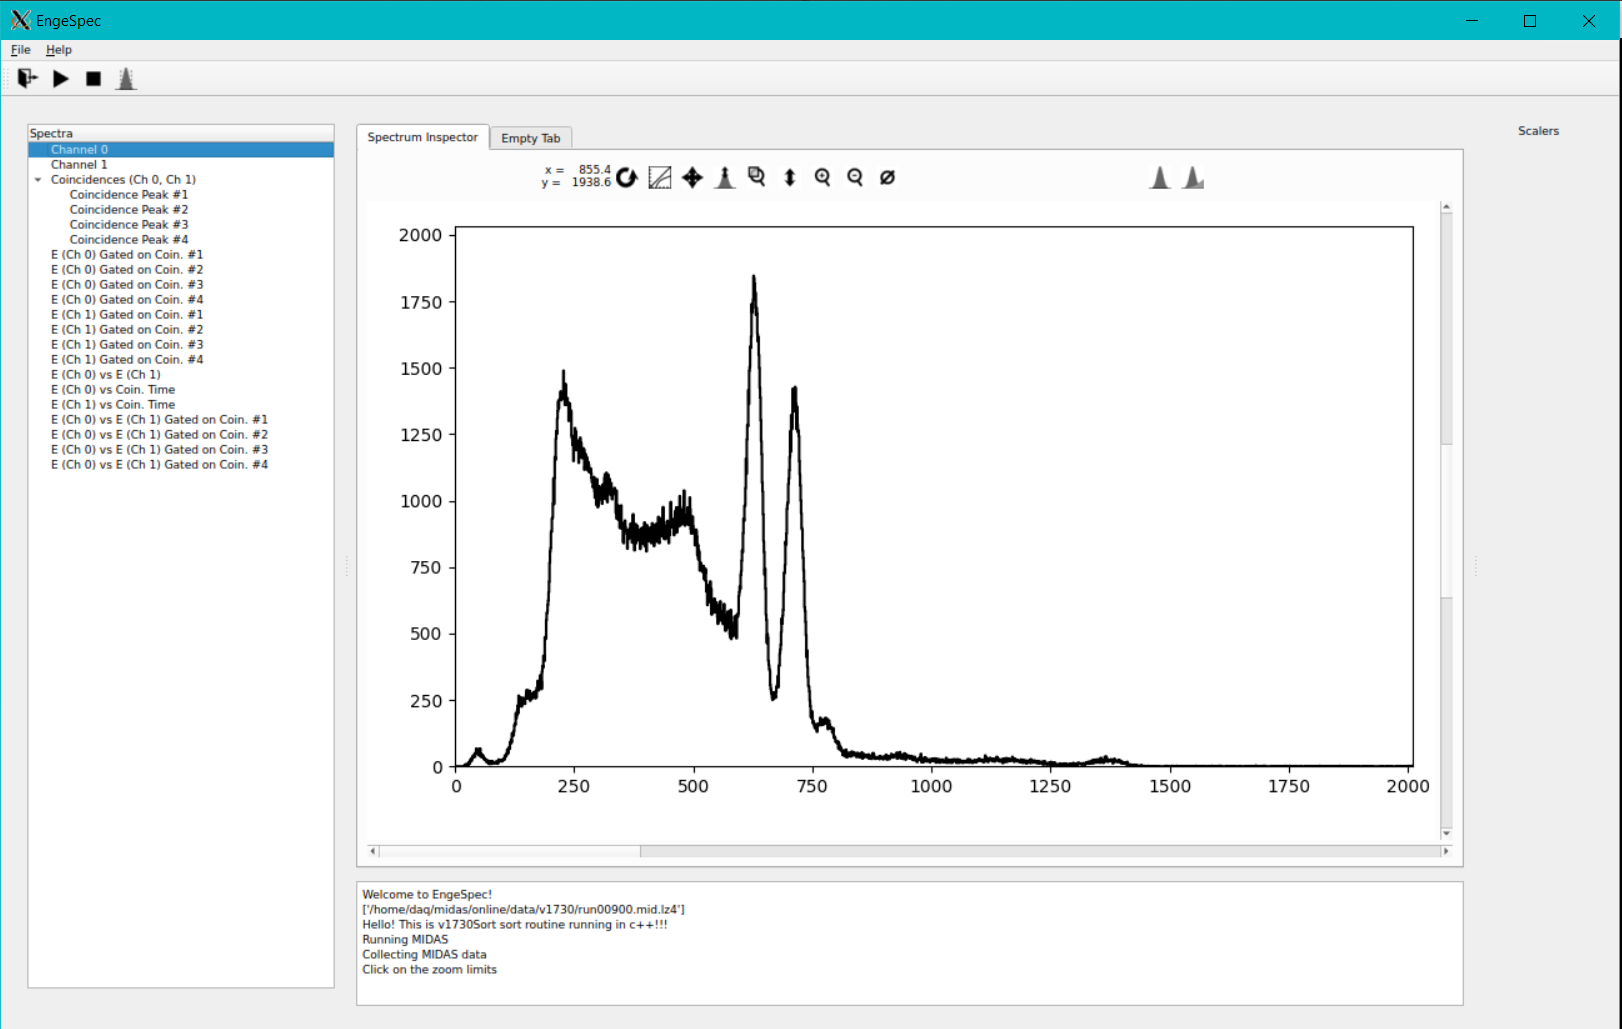
\includegraphics[scale=0.08]{Chapter-5/figs/Histogram_Co60.png}};
\node at (7.8,-4.5) {\footnotesize{Numerical Data}};
\hspace{1.6cm}

\end{tikzpicture}
\caption{\label{fig:new_electronics}The new method of converting detected particles and $\gamma$-rays into numerical data with a digitizer, replacing analog modules and the need for an ADC.}
\end{figure}

At TUNL, the users of the Enge Split-Pole Spectrograph will replace the focal plane detector analog modules with the CAEN V1730 digitizer and its associated Digital Pulse Processing (DPP) firmware algorithms. Fig. \ref{fig:upgrade} illustrates the difference between the traditional analog module setup versus the digitizer. Portability will be significantly improved, and a large amount of physical space will be freed up for other purposes. More importantly, the 14-bit digitizer will also provide enhanced energy and timing resolutions compared to the previous 12-bit ADC.

I led the development of a custom frontend DAQ software to accompany the digitizer, which uses MIDAS (Maximum Integrated Data Acquistion System) as the event-based DAQ. 
%The DAQ software used for the old system, NSCLDAQ, will no longer be supported soon, which is another incentive for the upgrades. 
In order to visualize the data collected by the DAQ, I helped in the development of a GUI, called \texttt{EngeSpec}, that is connected with MIDAS to provide live data visualization during experiments. It also has an offline mode for analysis with previously stored data. \texttt{EngeSpec} has several data analysis tools like curve fitting for gaussian and double-gaussian peaks, peak area calculation, and gating functionality. A C++ sort routine, called \texttt{EngeSort}, used with the old GUI has been revamped from Java for use with EngeSpec. As before, it sorts the data by detector channel and by observable into each given histogram. However, I added trigger and coincidence logic to be used with live signals for the focal-plane detector package, something that was previously performed by analog modules. Note that this has not yet been commissioned as of this thesis, but tests with the new digital DAQ that are not specific to the focal plane detector have already been successful and are presented in Section \ref{sec:DAQ_Tests}.

%\pagebreak

%\textcolor{white}{Empty space to force figure to top...}

\begin{figure}[t]
\centering
\begin{tikzpicture}[scale=1.4, every node/.style={transform shape}]
\hspace{0.3cm}
\node at (-3,0) {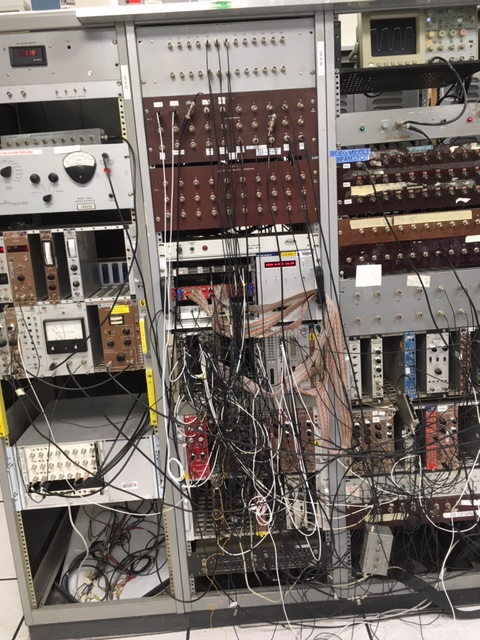
\includegraphics[scale=0.3]{Chapter-5/figs/Analog_Electronics.png}};
\node at (-3,-2.9) {\small{Analog Modules}};
\draw[->] (-0.5,0) -- (0.5,0);
\node at (0, 0.4) {\footnotesize{Upgrading}};
\node at (3,0) {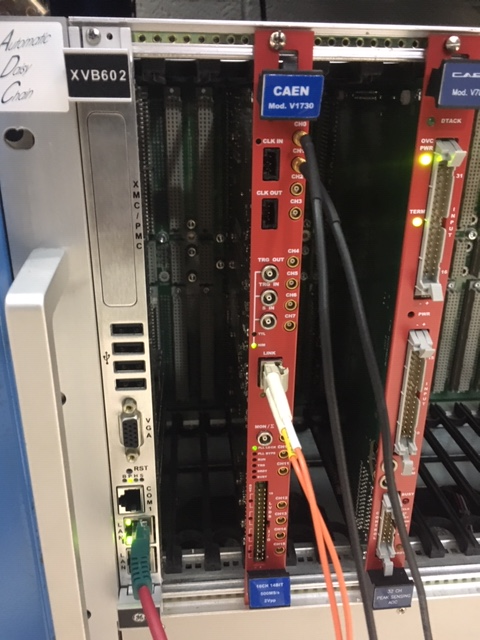
\includegraphics[scale=0.3]{Chapter-5/figs/Digitizer.png}};
\filldraw[fill = white] (4.1,-2.4) rectangle (5.9,-1.9);
\node at (5, -2.15) {\footnotesize{+ Software}};
\node at (3, -2.9) {\small{Digitizer}};
\end{tikzpicture}
\caption{\label{fig:upgrade}The CAEN V1730 Digitizer (pictured on the right), along with its associated DPP firmware and custom frontend DAQ software, is replacing the need for the unportable analog pulse-processing modules (pictured on the left) associated with the Enge focal-plane detector package at TUNL.}
\end{figure}

%%%%%%%%%%%%%%%%%%%%%%%%%%%%%%%%%%%%%%%%%%%%%%%%%%%%%%%%%%%%%%%%%%%%%%%%%%%%%%%

%\clearpage % This doesn't seem to separate the section because of the last figure
\section{Overview of the CAEN V1730 Digitizer} \label{sec:digitizer} 

This section provides a brief overview of how the CAEN V1730 digitizer functions, and the most important aspects of its Digital Pulse Processing (DPP) algorithms are discussed. Section \ref{sec:frontend} will then cover how to implement the algorithms via the frontend DAQ software. The version of the digitizer firmware we use is known as DPP-PSD, or Digital Pulse Processing for Pulse Shape Discrimination. The official CAEN DPP-PSD user manual is a comprehensive reference for details not covered in this chapter. 

%One of the main features of our version of the firmware is Pulse Shape Discrimination (PSD), which allows the user to distinguish between, for example, $\gamma$-ray and neutron events. Hence, it is known as the DPP-PSD firmware. The official CAEN DPP-PSD user manual is a useful reference for details not covered in this document.

\subsection{Digital Pulse-Processing Parameters} \label{subsec:DPP}

The V1730 digitizer is capable of sampling signals directly from detectors at a rate of 500 MS/s for each of its 16 input channels, corresponding to a time resolution of 2 ns per sample. Those samples are used by the DPP firmware in calculations of important quantities associated with a given signal, such as its baseline, energy, and time stamp. A typical sampled signal is shown in Fig. \ref{fig:trigger}, where parameters used by the DPP algorithms are summarized. These parameters are all user-defined and depend on the shape of the detector signals. One can use an oscilloscope or any waveform display software, such as \texttt{CoMPASS}, to approximate the parameters. For optimal resolution, it may be necessary to perform resolution tests for certain parameters over a range of values (see Section \ref{subsec:energy_resolution} for an example of this procedure).

%\subsubsection{Energy Calculation} \label{energy_calc}

\begin{figure}[t]
\centering
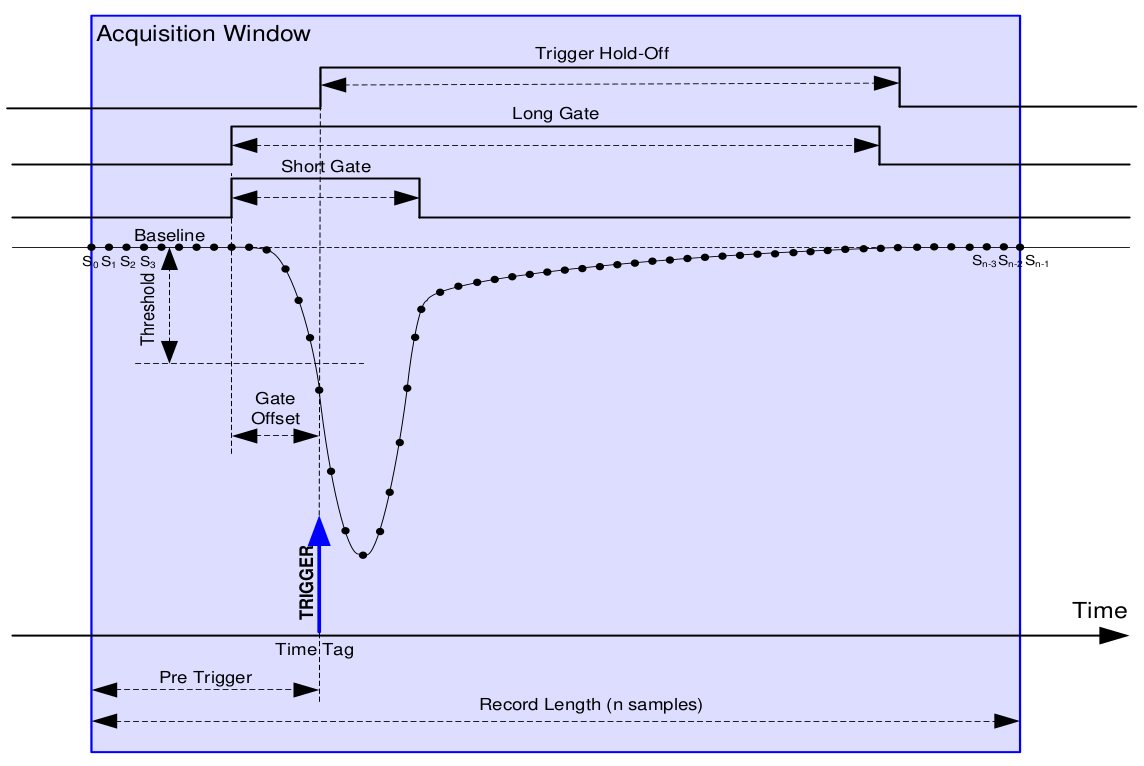
\includegraphics[width=6.5in]{Chapter-5/figs/trigger.png}
\caption{\label{fig:trigger}A signal sampled by the V1730 digitizer, summarizing the parameters used by the DPP algorithms. When the signal crosses the threshold value, the trigger fires, which primes the system for data acquisition.}
\end{figure}

A signal is triggered for data acquisition when it crosses the \emph{threshold} voltage, which should be set high enough to filter out low-energy noise, but low enough not to miss signals. When the trigger fires, the signal is delayed by the \emph{pre-trigger} width to prime for the energy calculation. Since the energy of a charged-particle event is proportional to the charge that it deposits, the digitizer calculates this charge, and therefore determines the (uncalibrated) energy, by integrating the signal voltage over time. The length of time used in the integration is a user-defined parameter known as the \emph{long gate}, and the integrated charge (i.e. uncalibrated energy) is denoted by $Q_{\textnormal{Long}}$. The energy integration begins a length of time before the trigger fires, known as the \emph{gate offset}, which must be less than the pre-trigger width. The purpose of the gate offset is to include the portion of the signal before the trigger in the energy integration. After the trigger fires, all other triggers from the same channel are inhibited during the \emph{trigger hold-off} width, which must last at least until the end of the long gate. After this width, the channel can accept new triggers. 

%Q: HOW DO EVENTS THAT ARE COINCIDENT EVEN GET TRIGGERED WHEN THEY SHOULD BE INHIBITED DURING THE TRIGGER HOLD-OFF WIDTH? 
%A: BECAUSE THE EVENTS THAT ARE COINCIDENT COME FROM DIFFERENT CHANNELS WITH THEIR OWN TRIGGER HOLD-OFF.

One of the most important quantities associated with the DPP algorithms is the baseline of the signal. The baseline is the reference value used for the energy calculation and to determine the threshold. This can either be a user-defined quantity, in which case it retains a fixed value, or the baseline can be dynamically calculated based on the average value of a user-defined number of samples during a moving time window. In the latter case, as shown in Fig. \ref{fig:baseline_calc}, the baseline freezes during energy integration, and the baseline calculation restarts after the trigger hold-off width, using the samples both before and after the freeze. This means the baseline calculation contributes almost no dead-time. Note that the threshold follows the baseline variations.

\begin{figure}[t]
\centering
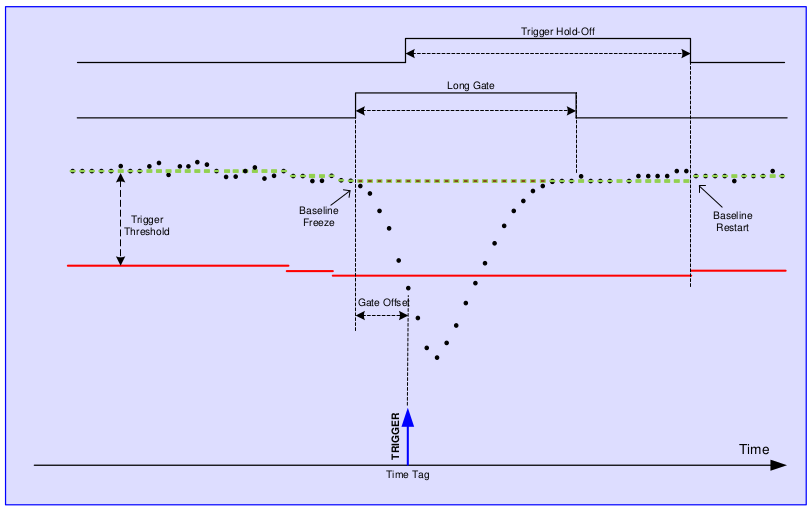
\includegraphics[width=6.5in]{Chapter-5/figs/baseline.png}
\caption{\label{fig:baseline_calc}The dynamic baseline calculation using the mean value of a user-defined number of samples in a moving time window. The baseline freezes during the energy integration of a signal that has been triggered.}
\end{figure}

The \emph{short gate} is a measure of the fast portion of the signal. This is used, in conjunction with the long gate, to discern between different types of particles, e.g. between gamma-rays and neutrons. The pulse shape discrimination (PSD) is a quantity that measures the ratio between the area of the tail of the signal and the area of the total signal, i.e.
\begin{equation*}
\textnormal{PSD} = \frac{Q_{\textnormal{Long}} - Q_{\textnormal{Short}}}{Q_{\textnormal{Long}}},
\end{equation*}
where $Q_{\textnormal{Long}}$ and $Q_{\textnormal{Short}}$ are the charge collected in the long gate and short gate during charge integration, respectively. Neutron events tend to have a distinctly higher PSD than gamma-ray events because they have larger tails. The option to collect the PSD for each event is currently not available in our frontend software, as we have other means of particle discrimination through post-processing.

The only parameter yet to be discussed in Fig. \ref{fig:trigger}, the \emph{record length}, is not used by our digitizer. The V1730 only operates in List mode, where the event data is stored, but the samples themselves are not. Some other CAEN digitizers can operate in Waveform mode, where the samples in the record length that make up the \emph{acquisition window} are stored to visualize the signals and the baseline with the appropriate CAEN software. However, the reduced amount of data transferred in List mode compared to Waveform mode keeps the dead-time of the system very low during runs.

\subsection{Time Stamp Determination} \label{subsec:time_stamp}

%\subsubsection{Leading Edge Discrimination} \label{LED}

By default, the timing of events in the DPP firmware is performed by \emph{leading edge discrimination} (LED), where a time stamp is given to each event the moment it crosses the trigger threshold. However, threshold triggering on the leading edge of signals causes well-known issues with timing, known as \emph{time walk}. Two signals exactly coincident, but with different amplitudes, will register different time tags using LED mode because the leading edge of the larger signal rises sooner. 

%\subsubsection{Constant Fraction Discrimination} \label{CFD}

A more precise way of determining signal time is by using \emph{constant fraction discrimination} (CFD), which can be enabled by the DAQ user instead of LED mode. This method assigns the time stamp to the moment the signal amplitude reaches a constant fraction of its total amplitude, allowing for timing to be independent of signal amplitude. As in traditional analog CFD modules, the digitizer takes the input signal and produces two new signals, one attenuated by a factor $f$ of the total amplitude and the other inverted and delayed by a time $d$. The two signals are summed together to form a bipolar pulse with a single \emph{zero-crossing}, which is taken as the time stamp of the event. Because of the finite sampling resolution of the digitizer, the exact zero-crossing location will always be located somewhere between two samples of the signal. The DPP firmware, by default, assigns the sample before the zero-crossing as the time stamp of the event, called the \emph{coarse time stamp}. This is usually sufficient, but for more precise timing it is also possible to assign the time stamp as the interpolated zero-crossing. The width between the coarse time stamp and the interpolated zero-crossing is called the \emph{fine time stamp}. If the user enables zero-crossing interpolation, the data for each event will take up more memory. Note that in the case of CFD mode, the threshold trigger serves the purpose of priming the system for CFD implementation rather than assigning a time stamp.

The time stamp for LED mode and the coarse time stamp for CFD mode are both referred to as the \emph{trigger time tag} in the DPP firmware, a 31-bit unsigned integer that has units equal to the time resolution of the digitizer, 2 ns. In CFD mode, the fine time stamp is a 10-bit unsigned integer, meaning the interpolated zero-crossing time stamp is a 41-bit unsigned integer (with a maximum value of $2^{31}$). The trigger time tag is stored by default, but the fine time stamp can be retrieved separately. Both the interpolated zero-crossing time stamp and the trigger time tag roll back to zero once they reach their maximum value of $2^{31}$, or $2 \times 2^{31}$ ns $\approx 4.295$ s. It is also possible to extend the rollback of the time stamps by an extra 16-bits by enabling the \emph{extended time stamp}. %\textcolor{red}{*CHECK THIS PARAGRAPH*} % THIS IS PROBABLY WRONG. MAKE SURE THIS PARAGRAPH IS CORRECT. I'M HAVING A HARD TIME WRAPPING MY HEAD AROUND THE ZERO-CROSSING TIME STAMP BEING 41-BITS, BUT HAVING A MAXIMUM (ROLL BACK) OF 2^31. TEST EXTRAS OUT USING CFD MODE TO SEE WHAT THE TRIGGER TIME TAG AND FINE TIME STAMPS LOOK LIKE.

\subsection{Event Readout Format} \label{subsec:memory}

Each of the 16 V1730 digitizer channels uses RAM to temporarily store event data. This memory is divided into \emph{memory buffers}, or \emph{aggregates}, that each contain data for up to 1023 events. The number of events per aggregate is programmable, but we have set this number to its maximum of 1023 as to optimize readout bandwidth. The drawback of this is that events are not available for readout until all 1023 events have been stored in an aggregate, unless the run is stopped before an aggregate becomes full. The total number of aggregates contained in the RAM is also programmable, but we have set this number to 8 due to the large size of each aggregate. The RAM for each aggregate is cleared after all aggregates have been read to make room for upcoming events. %\textcolor{red}{*CHECK THIS LAST PART*} % CHECK WITH RICHARD ABOUT THIS LAST PART

In reality, there are two types of aggregates for the V1730 memory organization. \emph{Channel aggregates} are what have been described so far, but there are also \emph{board aggregates}. Each channel aggregate is shared by two consecutive channels, i.e. channel 0 and channel 1, channel 2 and channel 3, etc. The sample of all channel aggregates is a board aggregate. The sample of all board aggregates is called the \emph{data block}. Since there are 16 channels in the V1730, there are up to 8 channel aggregates that comprise a board aggregate. If a channel aggregate contains no data, it is not included in the board aggregate. When data readout is performed, each successive channel aggregate is read at a time in a given board aggregate, and each successive board aggregate is read from the data block via a \emph{block transfer}.

\subsubsection{Channel Aggregate Event Format} %\label{channel_agg}

The channel aggregates are formatted for readout as in Fig. \ref{fig:ChannelAgg}. Each line represents a \emph{memory location}, consisting of a 32-bit integer (each bit is either a 0 or 1). Note that only 2 events are shown, and a full channel aggregate will contain 1023 events. The first two memory locations, SIZE and FORMAT, comprise the channel aggregate \emph{header}, which is common to all events in the aggregate. Beyond the header is data for each event in the aggregate. Our V1730 digitizer does not save individual samples, so every memory location that contains a sample, S$_{1}$, S$_{2}$, etc., does not appear for readout. Therefore, each event contains a maximum of 3 memory locations. These are the trigger time tag, EXTRAS, and the charges from the long and short gates, $Q_{\textnormal{Long}}$ and $Q_{\textnormal{Short}}$, respectively. EXTRAS contains extra information associated with CFD zero crossing interpolation. It is therefore omitted by default, unless the user has enabled CFD zero crossing interpolation. Note that if CFD mode is enabled, the trigger time tag is the coarse time stamp, associated with the sample before the zero crossing by default.

\begin{figure}[t]
\centering
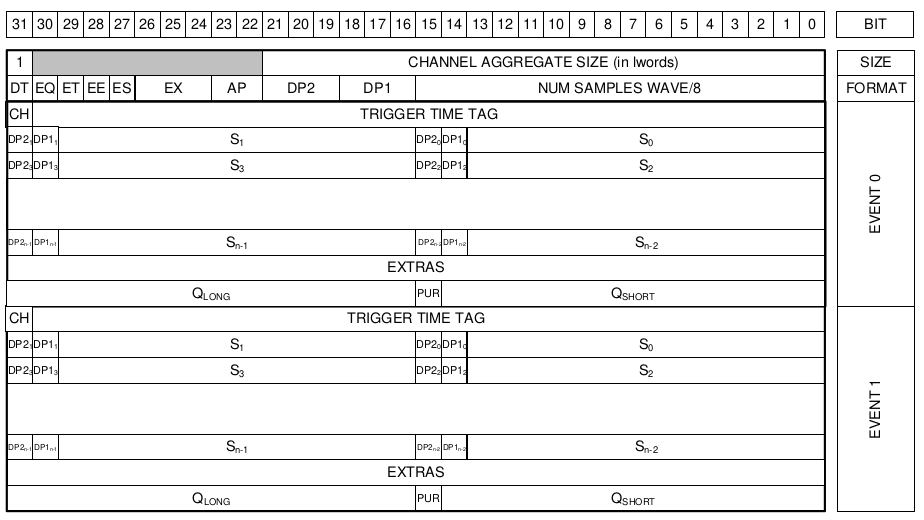
\includegraphics[width=6.5in]{Chapter-5/figs/ChannelAgg.png}
\caption{\label{fig:ChannelAgg}The data format for the first two events in a channel aggregate. Each memory location is 32-bits and is accessed during readout. Individual samples are not saved by our digitizer, so every 32-bit line that contains a sample, S$_{1}$, S$_{2}$, etc., is omitted. Each event therefore contains up to three memory locations. The channel aggregate itself has a header consisting of the first two memory locations, SIZE and FORMAT.}
\end{figure}

Not every bit in Fig. \ref{fig:ChannelAgg} will be discussed here. See the CAEN DPP-PSD manual for detailed information. However, the data most frequently accessed are as follows (from top to bottom in Fig. \ref{fig:ChannelAgg}). In the SIZE memory location, the CHANNEL AGGREGATE SIZE is the number of memory locations that are contained in the given channel aggregate, including itself and FORMAT. This can be useful for debugging and determining how many events are contained in the aggregate. In the FORMAT memory location, EX contains 3 bits that the user inputs (through functions in the frontend DAQ) to specify what the EXTRAS memory location outputs. If all 3 of these bits are 0, the EXTRAS memory location is omitted. In the event memory locations, CH specifies which channel the event came from in the couple (0 for even or 1 for odd). PUR is a flag that detects events whose energy was not evaluated correctly, e.g. from pile-up or event saturation. 

%Note that $Q_{\textnormal{Long}}$ and $Q_{\textnormal{Short}}$ are 16- and 15-bit signed integers, respectively, while the trigger time tag is a 31-bit unsigned integer. The reason $Q_{\textnormal{Long}}$ and $Q_{\textnormal{Short}}$ are signed integers is to clearly separate real events from noise. In the case of a pile-up event, for example,  

% (Don't use this:) Q_long and Q_short are signed integers and everything else is an unsigned integer, but the details are probably not important to include... Except that it explains the 65535 spike issue.

\begin{figure}[t]
\centering
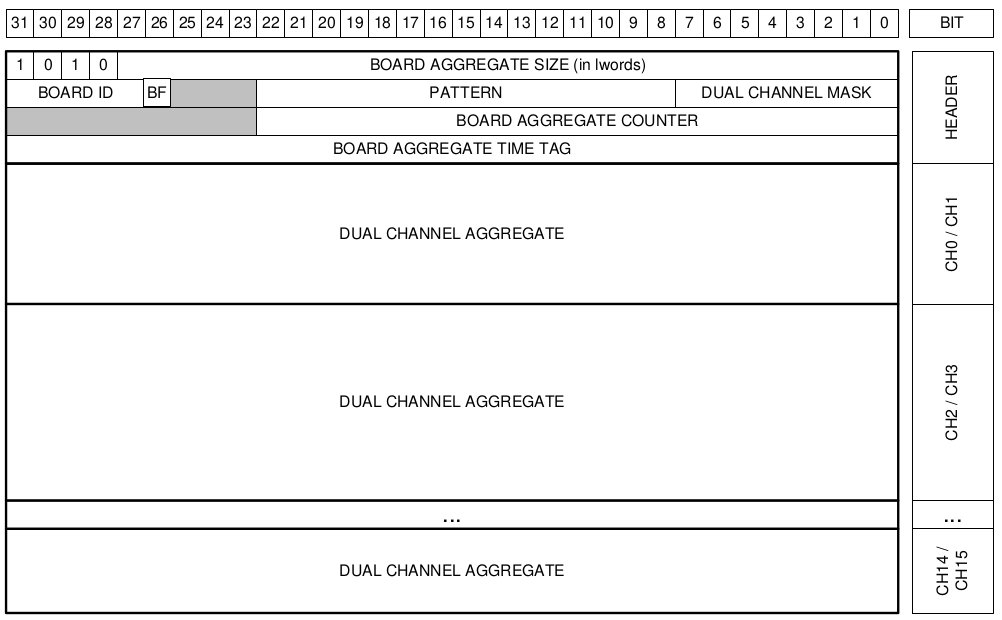
\includegraphics[width=6.5in]{Chapter-5/figs/BoardAgg.png}
\caption{\label{fig:BoardAgg}The data format for a board aggregate, consisting of up to 8 channel aggregates and 4 memory locations making up the header. Each memory location is 32-bits and is accessed during readout.}
\end{figure}

\subsubsection{Board Aggregate Event Format} %\label{board_agg}

The board aggregates are formatted for readout as in Fig. \ref{fig:BoardAgg}. Each board aggregate contains up to 8 channel aggregates and has 4 memory locations making up the header. Each channel aggregate that has data contributes all of its memory locations to the board aggregate in the order shown in Fig. \ref{fig:BoardAgg}. Channel aggregates with no data do not contribute to the board aggregate.

Again, only the most important values in the board aggregate will be discussed here. The BOARD AGGREGATE SIZE is analogous to the CHANNEL AGGREGATE SIZE in that it is the total number of memory locations contained in the board aggregate, including all of the memory locations in the channel aggregates that comprise it. The DUAL CHANNEL MASK corresponds to the channel couples participating to the board aggregate. THE BOARD AGGREGATE COUNTER gives the current board aggregate count. The BOARD AGGREGATE TIME TAG gives the time that the board aggregate was created. This is not a physical quantity, but can be useful for debugging.

%\subsubsection{Data Block} \label{data_block}

%%%%%%%%%%%%%%%%%%%%%%%%%%%%%%%%%%%%%%%%%%%%%%%%%%%%%%%%%%%%%%%%%%%%%%%%%%%%%%%

%\pagebreak
\section{Frontend DAQ Software} \label{sec:frontend}

%\subsection{V1730 Registers} \label{subsec:registers}

The CAEN V1730 digitizer firmware uses Digital Pulse Processing (DPP) algorithms, which are implemented in the Field-Programmable Gate Array (FPGA) of the digitizer board. The DPP algorithms and settings can therefore be programmed by the user. This is performed by accessing and writing values to 32-bit wide \emph{registers}, which have distinct hexadecimal addresses. For example, setting the width of the long gate for channel 0 amounts to writing the long gate value (as a 16-bit integer) into the Long Gate Width register specific to channel 0, which has the address 0x1058. All of the registers that the user can access are documented in the official V1730 DPP-PSD Registers manual. %\textcolor{blue}{[Ref]}. %\ref{V1730 DPP Registers} 
Some of the most important registers will be highlighted in the next section, which can easily be adjusted with the use of a settings file.

%\subsection{User Settings} \label{settings}

An important aspect of our custom DAQ software is to provide a simple way of changing user-defined settings (DPP paramters) without the user having to manually keep track of register values. In the DAQ software, the different settings are implemented via C++ functions writing the given parameter values into the appropriate register when executed. The function definitions are stored in the C file v1730DPP.c, while the functions are executed in the frontend C++ file fev1730-DPP.cxx. Almost all settings the user would ever need to specify are listed in the settings file, settings-DPP.dat, shown in Fig. \ref{fig:settings_file}, allowing for quick changes to be made. This file is read, and the settings are applied, by the frontend file. Therefore, the frontend file must be executed with each change to the settings file. Any additional, less common settings can be added to the settings file at any point with ease.

\begin{figure}[t]
\centering
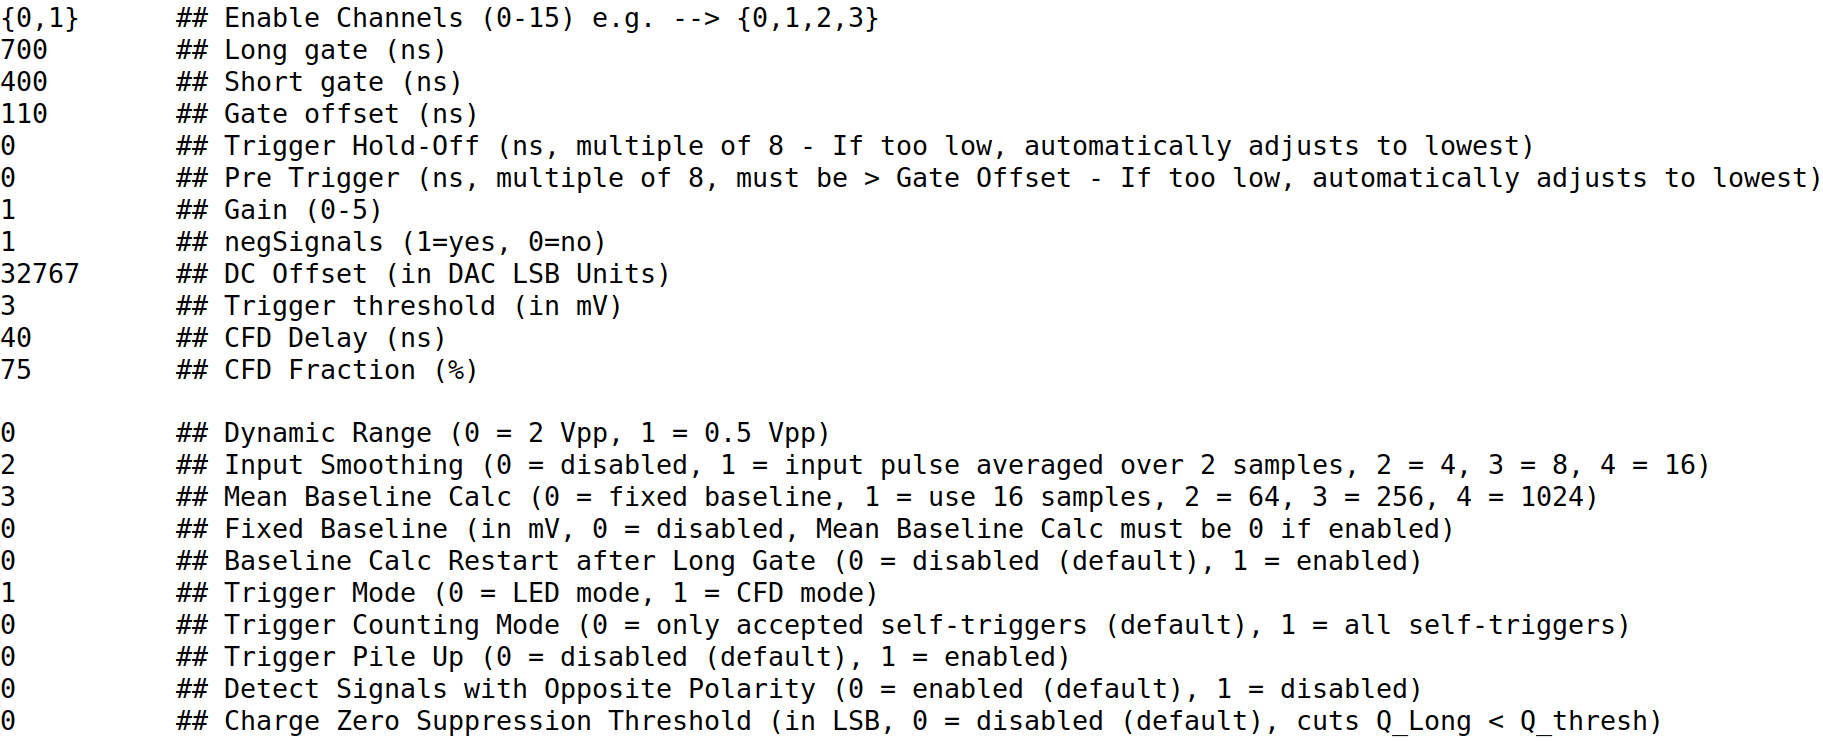
\includegraphics[width=6.5in]{Chapter-5/figs/settings_file4.png}
\caption{\label{fig:settings_file}The settings file, settings-DPP.dat, where the most common user-defined DPP parameters are adjusted. It is unlikely any other internal setting is needed, but implementing new V1730 register settings has been made simple.}
\end{figure}

%\subsubsection{Settings Determined from Oscilloscope Signals} \label{oscilloscope}

%\subsubsection{LED vs. CFD Mode} \label{LED_CFD}

%\subsubsection{Gain} \label{gain}

%\subsubsection{Mean Baseline Calculation} \label{mean_baseline_calc}

%\subsubsection{Input Smoothing} \label{smoothing}

%\subsubsection{Coincidences} \label{coincidences}

%Coincidences of events from different channels are obtained by subtracting their time tag values. Our DAQ has a coincidence feature that automatically deterimines coincidences between specified channels and can display coincidence spectra on the EngeSpec GUI (see

%\subsubsection{Other Settings} \label{other_settings}

%\subsection{MIDAS Data Collection} \label{MIDAS} % Don't include this
%\subsection{Making Changes and Starting Runs}



%%%%%%%%%%%%%%%%%%%%%%%%%%%%%%%%%%%%%%%%%%%%%%%%%%%%%%%%%%%%%%%%%%%%%%%%%%%%%%%

%\pagebreak
%\section{EngeSpec GUI} \label{sec:EngeSpec}

%\subsection{Overview of EngeSpec Operation}

%\subsubsection{Sort Routine: EngeSort}

%\subsubsection{Online MIDAS Runs}

%\subsubsection{Offline MIDAS Runs}

%\subsection{GUI Features}

%\subsubsection{Histogram Display}

%\subsubsection{Curve Fitting}

%\subsubsection{Coincidences}

%\subsubsection{Gating}

%%%%%%%%%%%%%%%%%%%%%%%%%%%%%%%%%%%%%%%%%%%%%%%%%%%%%%%%%%%%%%%%%%%%%%%%%%%%%%%

%\pagebreak
\section{Testing the Digital Data Acquisition System} \label{sec:DAQ_Tests}
%\subsection{Resolution Tests with a NaI Detector} \label{subsec:resolution}

I performed the initial tests on the digital DAQ and DPP settings by measuring both the energy resolution and timing resolution using NaI(Tl) scintillation detectors. Note that a commissioning experiment has yet to take place for the new digital DAQ at the Enge Split-Pole Spectrograph using the focal plane detector package. However, these initial tests proved insightful in the development of the sort routine that will be implemented for the focal plane detector signals when the commissioning experiment takes place. This section showcases the results of the resolution tests, where optimal DPP settings were determined, and several features that were added to the \texttt{EngeSpec} sort routine.

\subsection{Energy Resolution Tests with $^{152}\mathrm{Eu}$} \label{subsec:energy_resolution}

%and 1112.076(3) keV
The extraction and analysis of the integrated charge $Q_{long}$ is one of the most important goals in testing the DAQ because it represents the energy deposited in the detector. $Q_{long}$ is extracted from its memory location in each event collected over all channel aggregates and board aggregates, with reference to Figs. \ref{fig:ChannelAgg} and \ref{fig:BoardAgg}, respectively. The energy spectrum is then obtained by sorting the event data in the \texttt{EngeSpec} sort routine and incrementing a histogram with $Q_{long}$ values. In the present test, the radioisotope $^{152}$Eu was used along with a NaI(Tl) scintillator to analyze the $\gamma$-ray energies resulting from $\beta$-decay. The $^{152}$Eu $\gamma$-ray spectrum, incremented by the raw $Q_{long}$ values, is represented in Fig. \ref{fig:Eu152_spectrum}. Four calibration peaks are clearly visible. The right-most peak corresponds with the 1408.013(3) keV state \cite{IAEA2007}, which will be the focus of the resolution tests, since it is the most isolated. 

\begin{figure}[t]
\centering
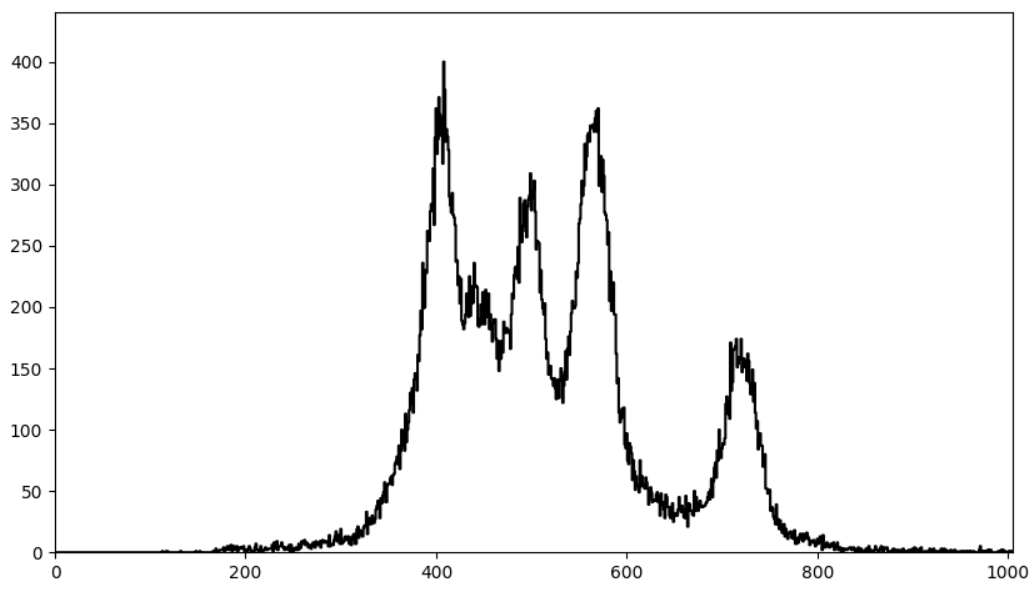
\includegraphics[width=6.5in]{Chapter-5/figs/Eu152_Spectrum.png}
\caption{\label{fig:Eu152_spectrum}The $^{152}$Eu $\gamma$-ray spectrum as a result of $\beta$-decay. The raw $Q_{long}$ value is given on the $x$-axis and the number of counts in each bin is given on the $y$-axis. The largest four $\gamma$-ray peaks are shown, where the right-most one is the 1408 keV peak used for the energy resolution analysis.}
\end{figure}

To measure the energy resolution, the full-width at half max (FWHM) and the centroid of the 1408 keV calibration state was determined by fitting a gaussian distribution plus a background line in the EngeSpec GUI. An energy calibration was performed with the other $^{152}$Eu calibration states, and the resulting energy distribution was used to calculate the relative resolution $R$ as a percentage
\begin{equation}
R = 100 \times \mathrm{FWHM}_{E}/E_{\mathrm{c}} \,\, [\mathrm{in} \, \, \%],
\end{equation}
where $\mathrm{FWHM}_{E}$ is in terms of calibrated energy and $E_{\mathrm{c}}$ is the calibrated peak energy.

The impact of the DPP parameters on the resolution was tested by varying a single DPP parameter and calculating the new resolution for each step. This was first performed for the long gate parameter, since this has the most direct link to $Q_{long}$, as it defines the gate for energy integration. Similarly, the gate offset parameter was varied next, since this also plays a role in the energy integration before the trigger fires. The results of the resolution tests for these parameters are given in Fig. \ref{fig:resolution_plots}. The long gate shows a clear minimum (i.e. best) resolution of about 5.5$\%$ for 500 ns. This corresponds to the true size of the signals when analyzed with an oscilloscope. The sharp rise as gate sizes become smaller than this makes physical sense, as the integration range begins to stop before reaching the end of the signal. However, the steady rise at gate sizes larger than the signal itself is interesting. One would think that a larger integration range would not play a significant role, considering the additional contribution to the charge should be negligible. It appears this is not the case, however. The likely scenario is that the baseline for the signal is slightly unparallel to the true, virtual baseline, so that more and more charge is accumulated at large gate size. The conclusion is that the raw signals should always be investigated with an oscilliscope and the long gate adjusted accordingly before scientific runs.

\begin{figure}[t]
\centering
\begin{tikzpicture}[scale=0.95, every node/.style={transform shape}]
\node at (-0.8,0) {\llap{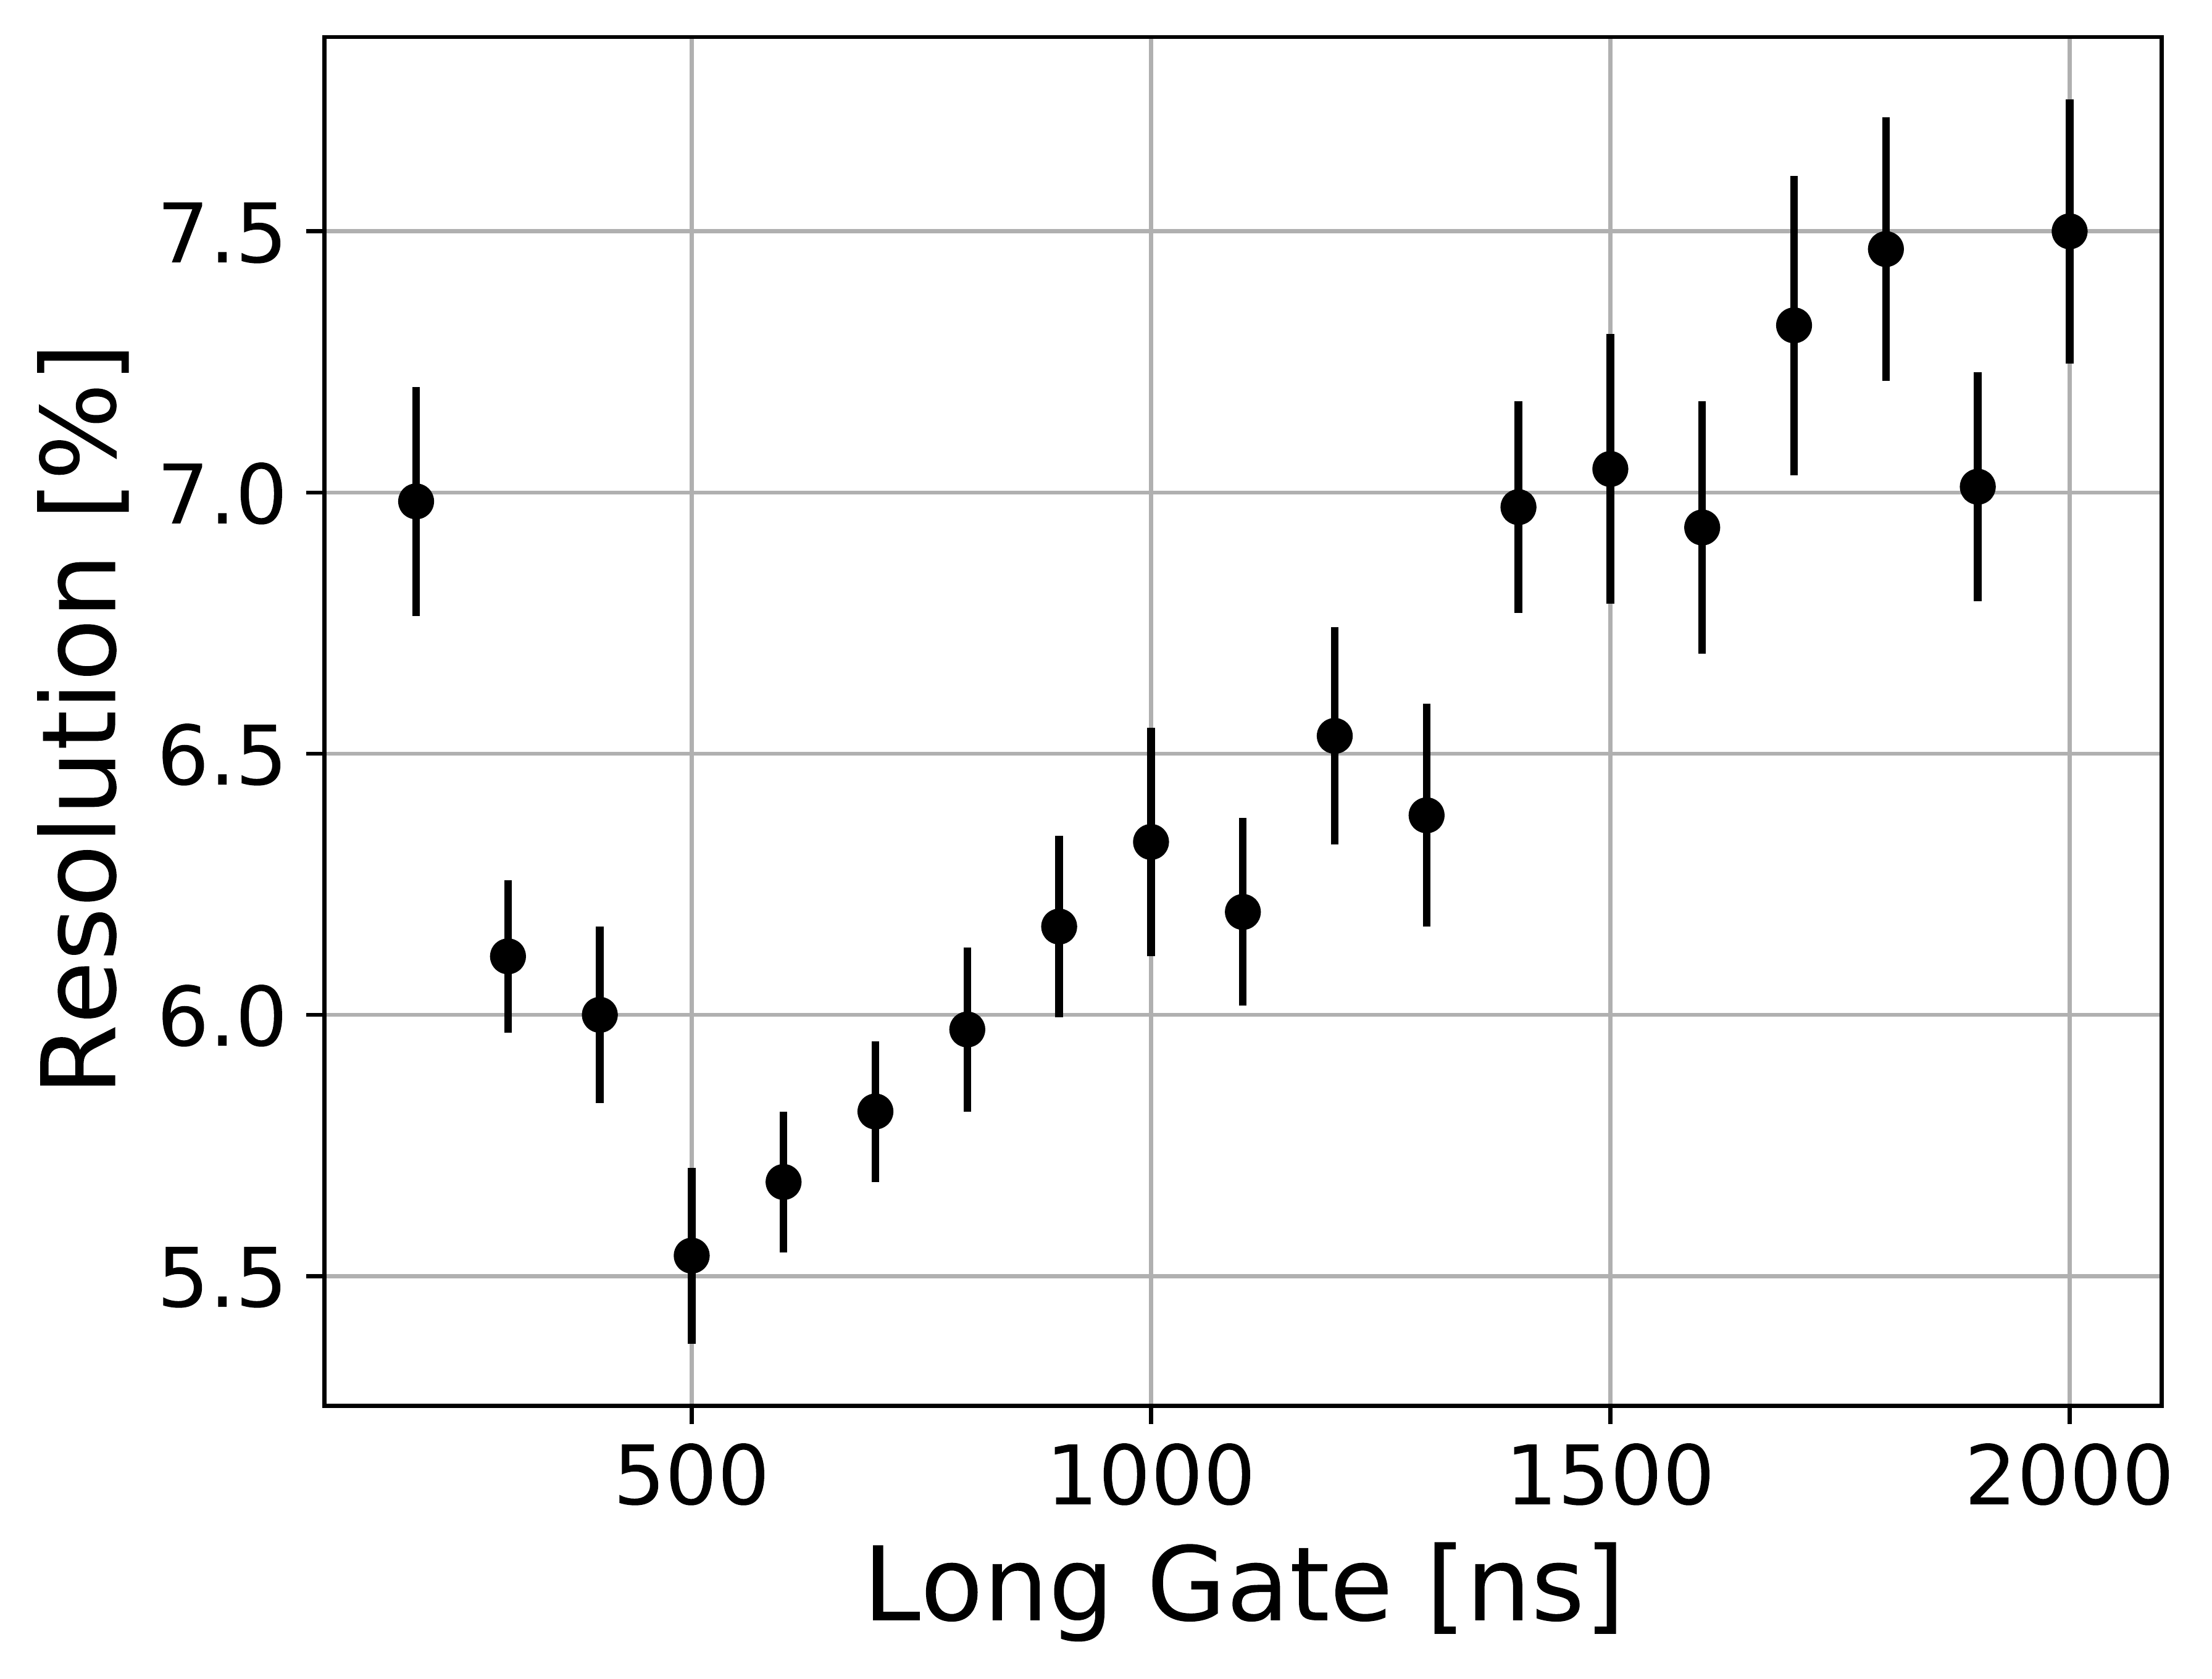
\includegraphics[width=\textwidth/2]{Chapter-5/figs/LongGate.png}}};
\node at (-0.2,0) {\rlap{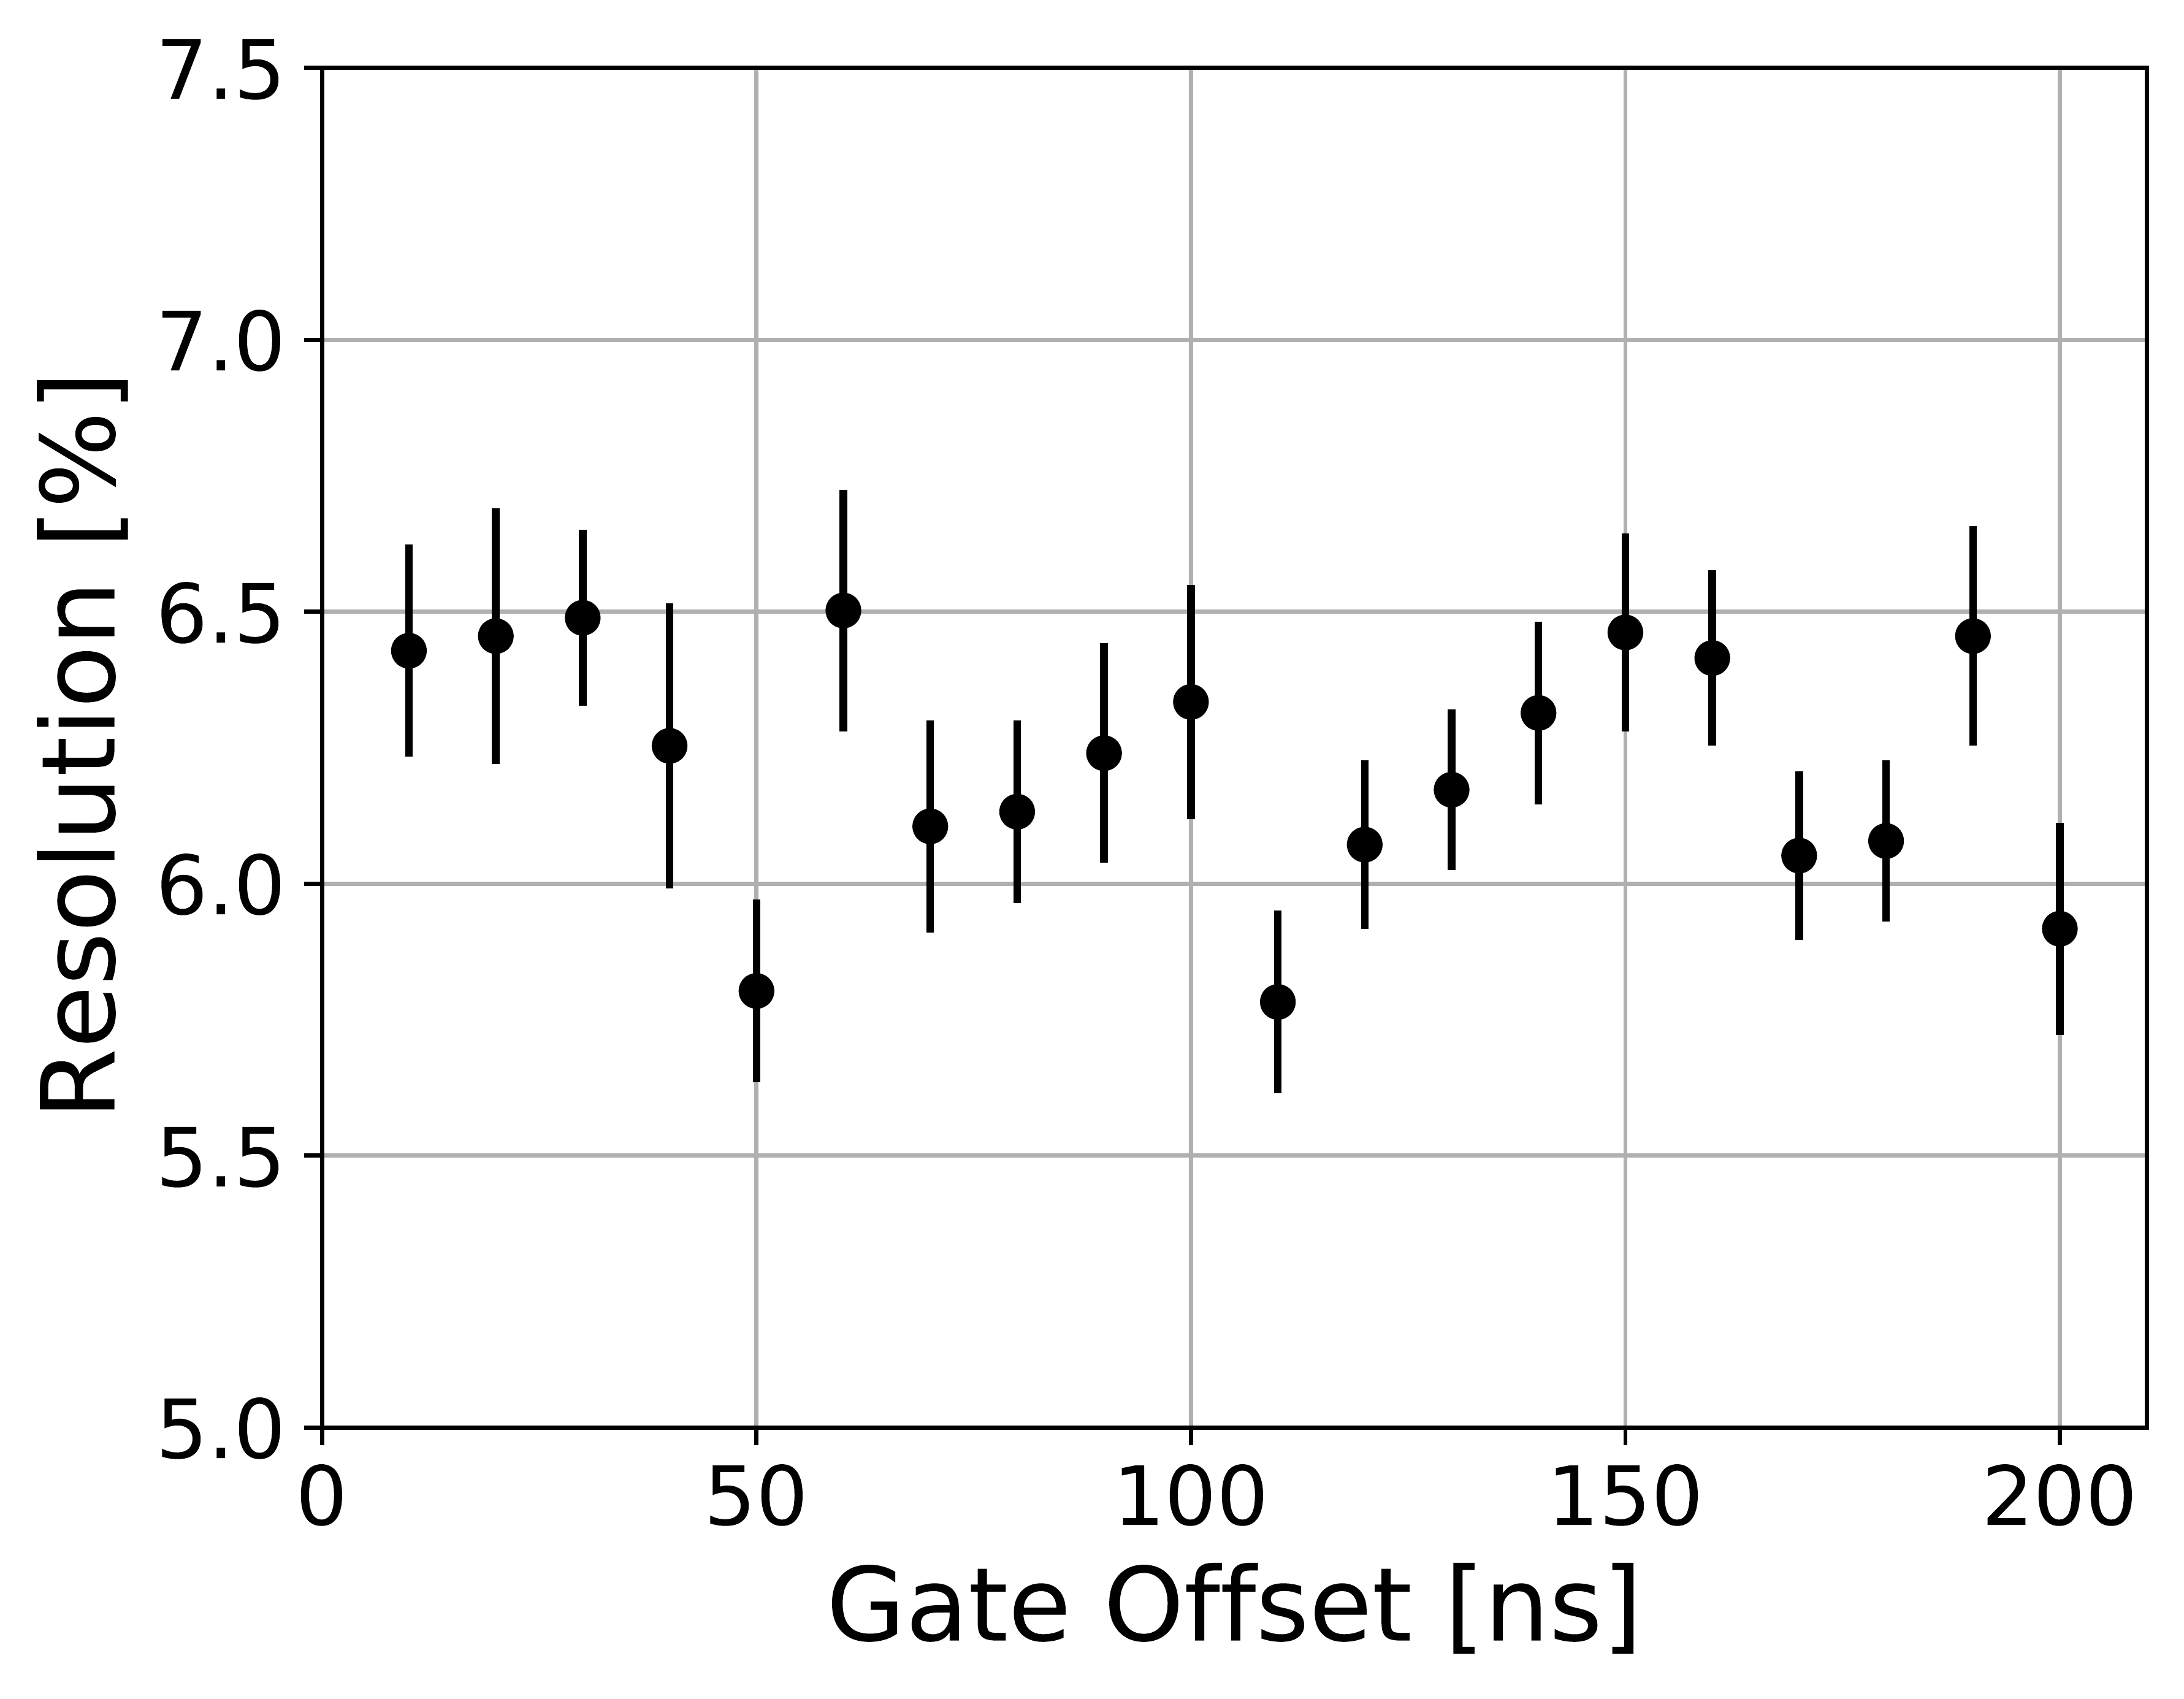
\includegraphics[width=\textwidth/2]{Chapter-5/figs/GateOffset.png}}};
\end{tikzpicture}
\caption{\label{fig:resolution_plots}Resolution tests of the long gate (left) and gate offset (right) DPP parameters for the 1408 keV $^{152}$Eu calibration state.}
\end{figure}

The resolution distribution for the gate offset parameter is more complicated and perhaps less insightful. There are two minima, at 50 ns and 110 ns, but the distribution rises abruptly on either side. This likely indicates that the resolution is not sensitive to this parameter, and the plot only shows statistical scatter. The quick fall time in the oscilloscope signals for this radiation source is likely the reason the gate offset has little impact.

These resolution tests were performed for many of the other parameters listed in Table \ref{fig:settings_file} as well, and there were minor improvements. They will not be described here for brevity, but the optimum parameters were found to be gain = 1, mean baseline calculation = 3, and input smoothing = 2. The trigger threshold did not have a clear minimum, and no other parameters were tested.

\subsection{Timing Resolution Tests with $^{60}\mathrm{Co}$} \label{subsec:timing_resolution}

The timing resolution for the digital DAQ was tested by measuring coincidences. For this purpose, two NaI(Tl) scintillation detectors were needed. A $^{60}$Co source was used this time because of its simplicity, and no energy calibration was needed. The $\gamma$-ray distribution for one of the detectors is shown in Fig. \ref{fig:Hist_60Co}, where the full \texttt{EngeSpec} GUI is shown. The 1332 keV and 1173 keV peaks are clearly visible. Coincidences between the two detectors are handled entirely by the \texttt{EngeSpec} sort routine. The development of the coincidence feature in \texttt{EngeSpec} is detailed in Section \ref{subsec:coincidences}.

\begin{figure}[t]
\centering
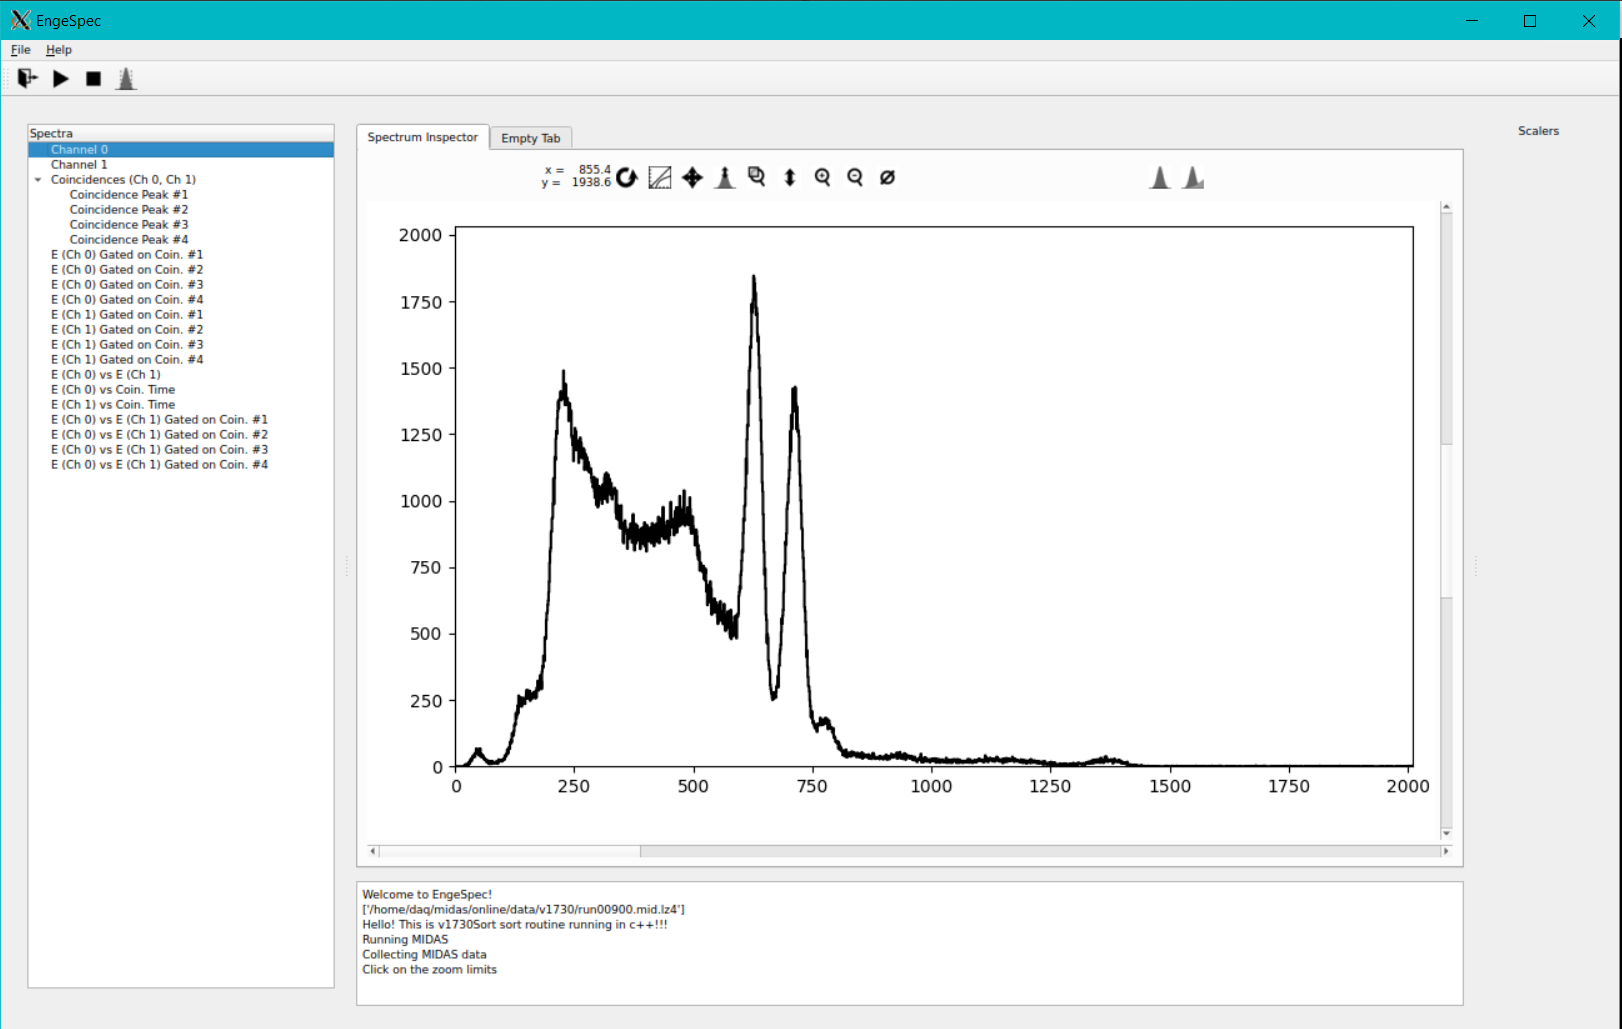
\includegraphics[width=6.5in]{Chapter-5/figs/Histogram_Co60.png}
\caption{\label{fig:Hist_60Co}The $^{60}$Co $\gamma$-ray spectrum shown with the \texttt{EngeSpec} GUI.}
\end{figure}

\begin{figure}[!p]
\centering
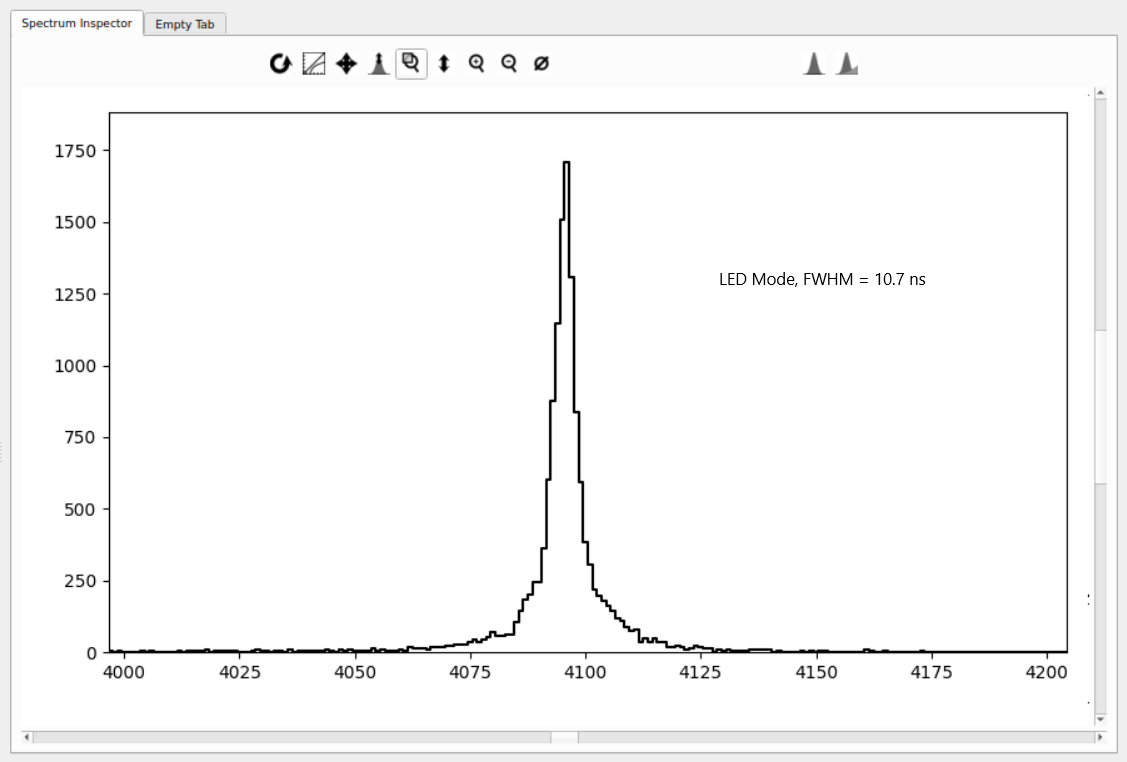
\includegraphics[width=5in]{Chapter-5/figs/Co60_LED_Coin.png}
\caption{\label{fig:Co60_LED_Coin}The coincidence histogram using the LED time stamp determination mode. The channels on the $x$-axis span from 0 to 8196, where the $\Delta t = 0$ condition has been shifted to the center, at channel 4096. The FHWM is found to be 10.7 ns for this case.}
\end{figure}

\begin{figure}
\centering
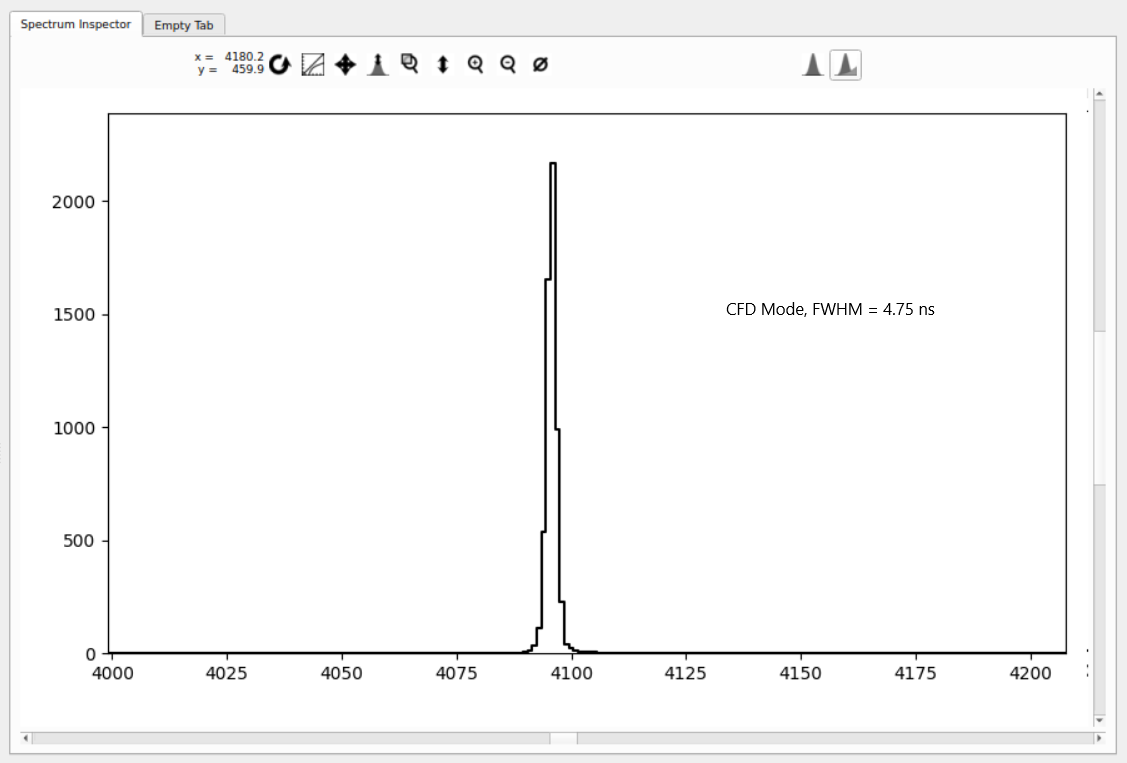
\includegraphics[width=5in]{Chapter-5/figs/Co60_CFD_Coin.png}
\caption{\label{fig:Co60_CFD_Coin}The coincidence histogram using the CFD time stamp determination mode. The FWHM is 4.75 ns for this case.}
\end{figure}

At the beginning of these tests, the default time stamp determination had been set to leading edge discrimination (LED), or LED mode, described in Section \ref{subsec:time_stamp}. Unsurprisingly, the timing resolution was clearly impacted as a result. Fig. \ref{fig:Co60_LED_Coin} shows a histogram of the coincidences obtained with LED mode, where the $x$-axis spans the channels 0 to 8196, and the time differences have been scaled so that $\Delta t = 0$ corresponds to channel 4096. The trigger time tags themselves have a resolution of 2 ns, so each channel in the histogram represents 2 ns. The coincidence fit is found to have a FWHM of 10.7 ns. The base of the peak appears to be broad and is contributing to the width. Using constant fraction discrimination (CFD mode), the result significantly narrows. This is seen in Fig. \ref{fig:Co60_CFD_Coin}, where the FWHM is 4.75 ns. Hence, the timing resolution for the digital DAQ using CFD mode is over twice as good as that of LED mode.

%Upon inspection of the compressed 512 x 512 channel 2D histogram for E vs $\Delta t$ in Fig. \ref{fig:Co60_LED_EvsT0}, the problem can be observed. This histogram shows $\Delta t$ on the $x-$axis and E on the $y$-axis. The density is represented by color. It is clear that the two bright spots at the top of the histogram correspond to the 1332 keV and 1173 keV peaks.

%LED mode has caused the values of $\Delta t$ 

%Fig. \ref{fig:Co60_LED_EvsT0} shows this effect, where coincidences are displayed in the form of a 512 x 512 channel 2D energy vs. time difference $\Delta t$ histogram. The $x$-axis has been offset so that the $\Delta t = 0$ case is at the center of the histogram, at channel 256. The $y$-axis is energy, and it is clear that the two bright spots at the top of histogram correspond to the 1332 keV and 1173 keV peaks.

%For the timing resolution test, a $^{60}$Co source was used because of its much more sharp 1332 keV and 1173 keV calibration peaks. The $\gamma$-ray energy distribution for one of the detectors is shown in Fig. \ref{fig:Hist_60Co}, where the full \texttt{EngeSpec} GUI is shown. Coincidences are 

%\begin{figure}[t]
%\centering
%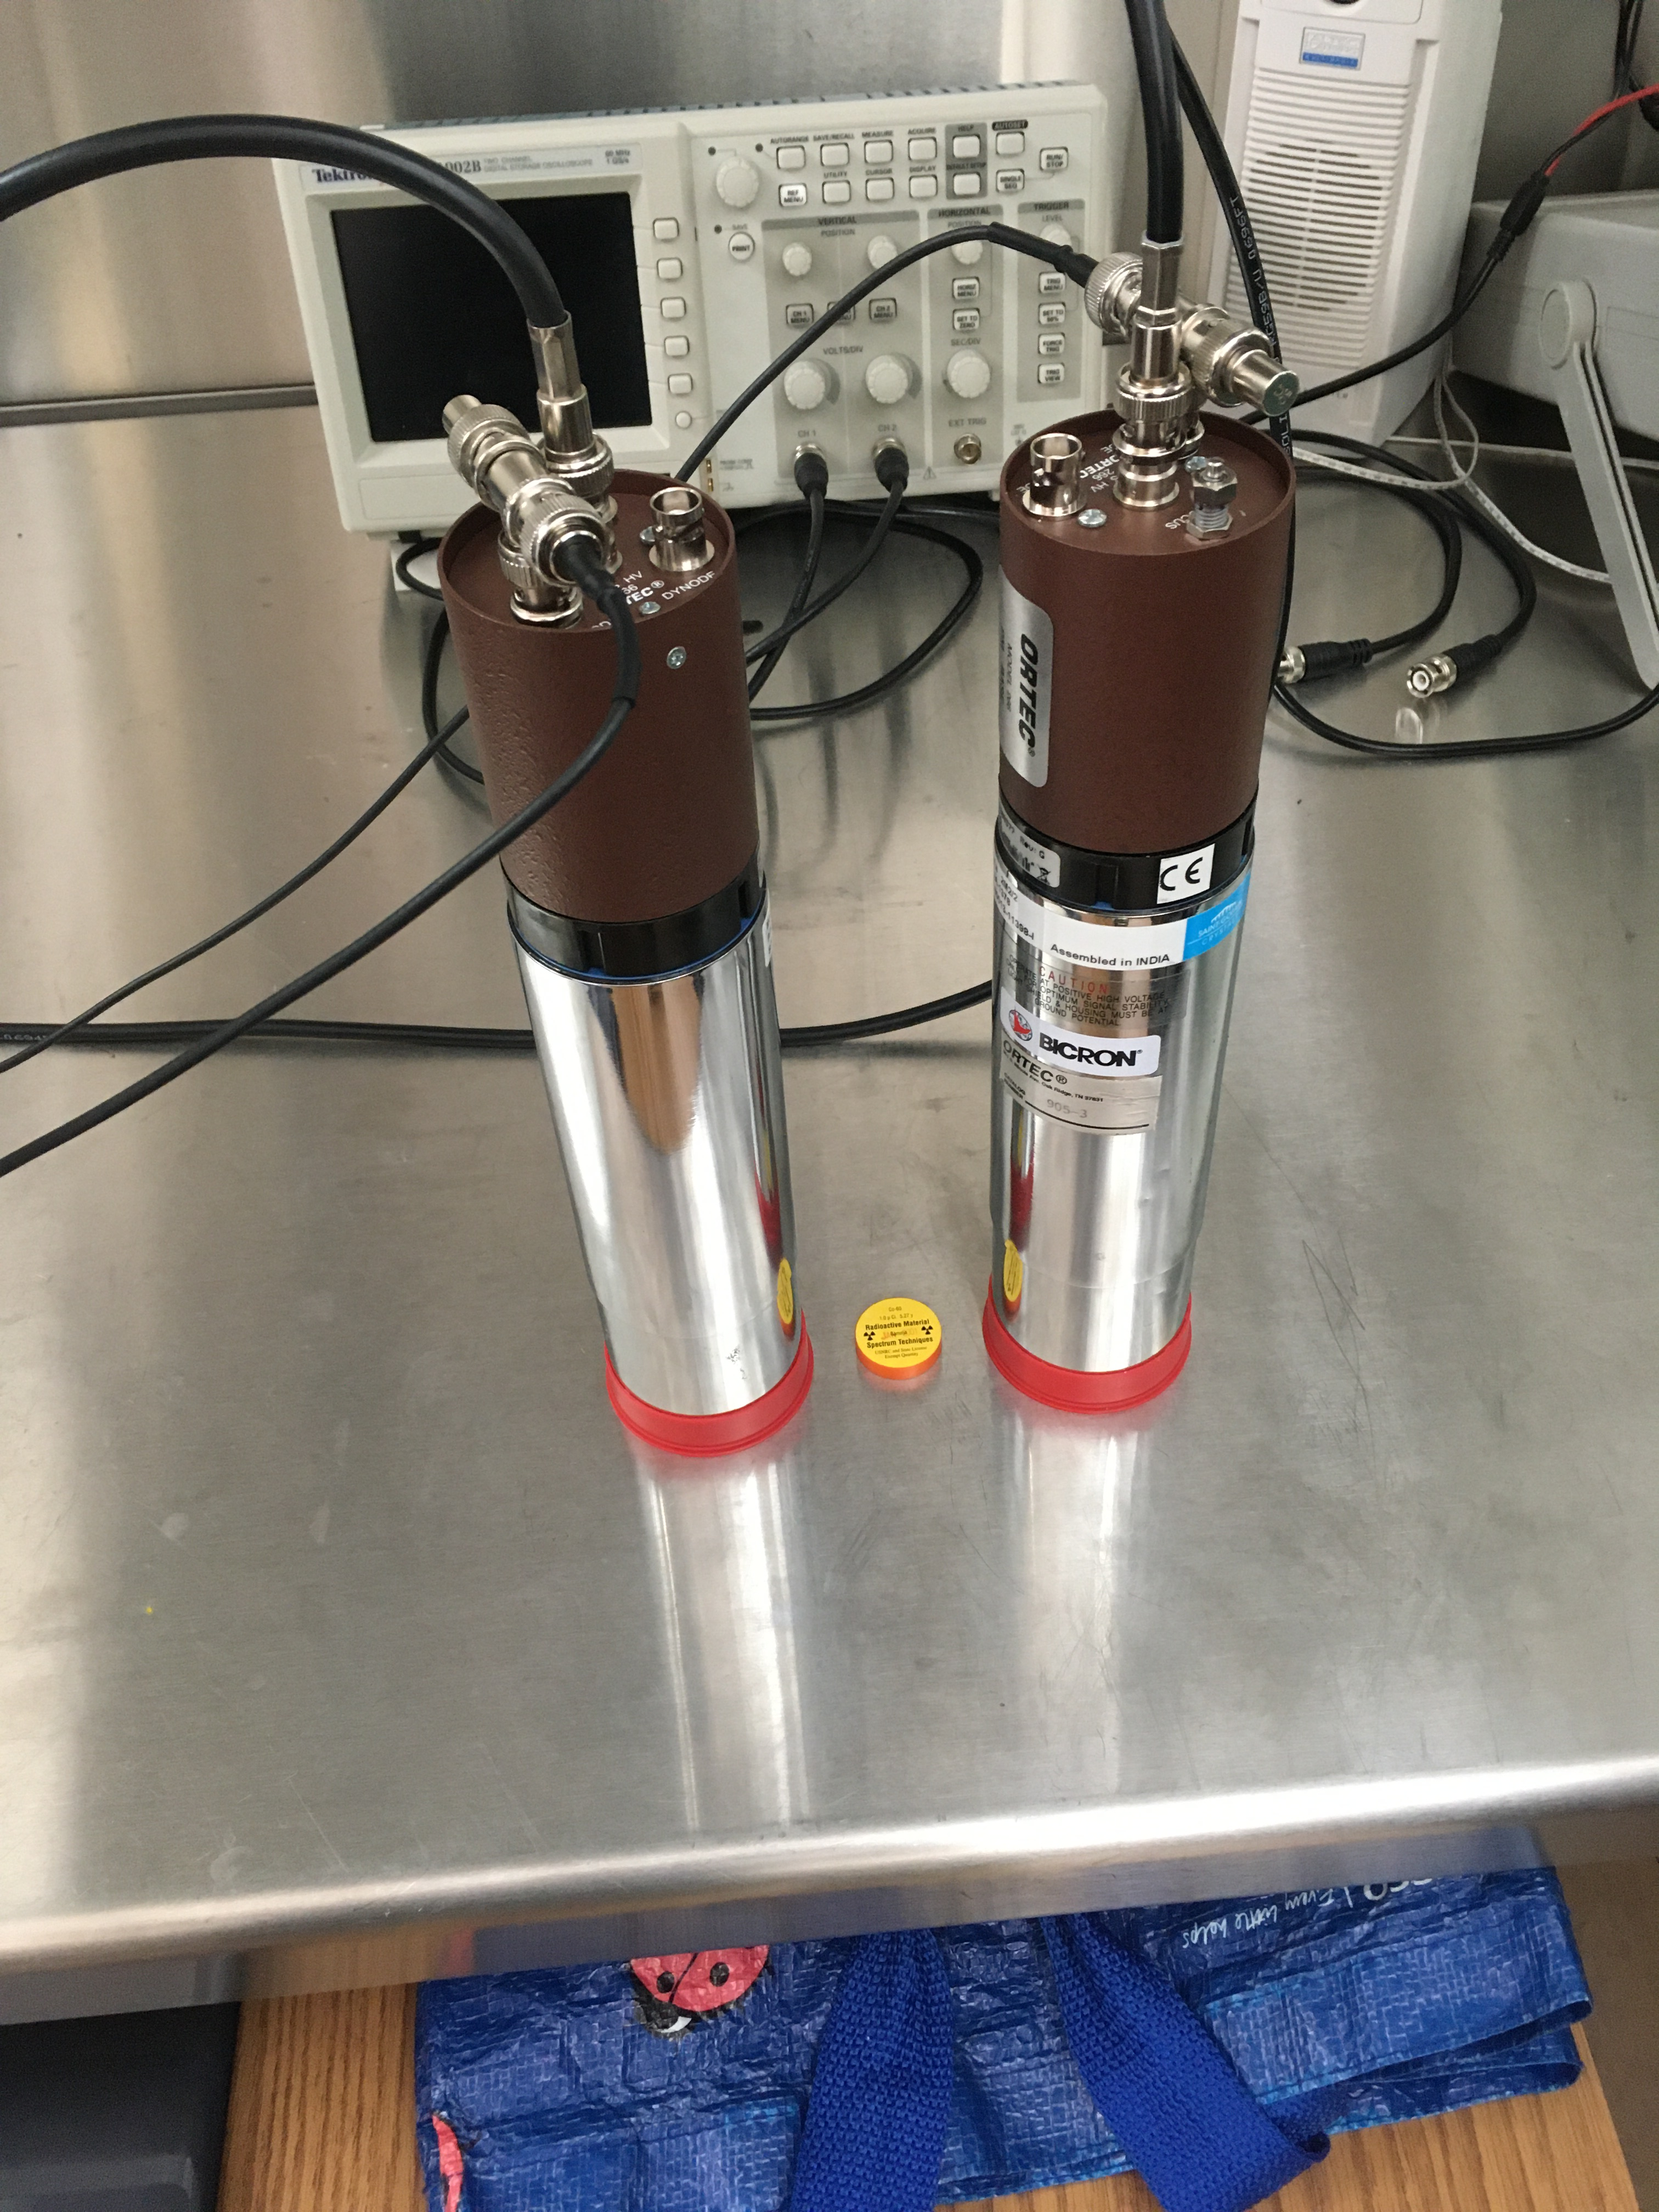
\includegraphics[width=5.5in]{Chapter-5/figs/NaI.JPG}
%\caption{\label{fig:NaI}The $^{60}$Co coincidence setup testing the timing resolution of the digital DAQ with two Ortec NaI(Tl) scintillation detectors.}
%\end{figure}

%\begin{figure}[t]
%\centering
%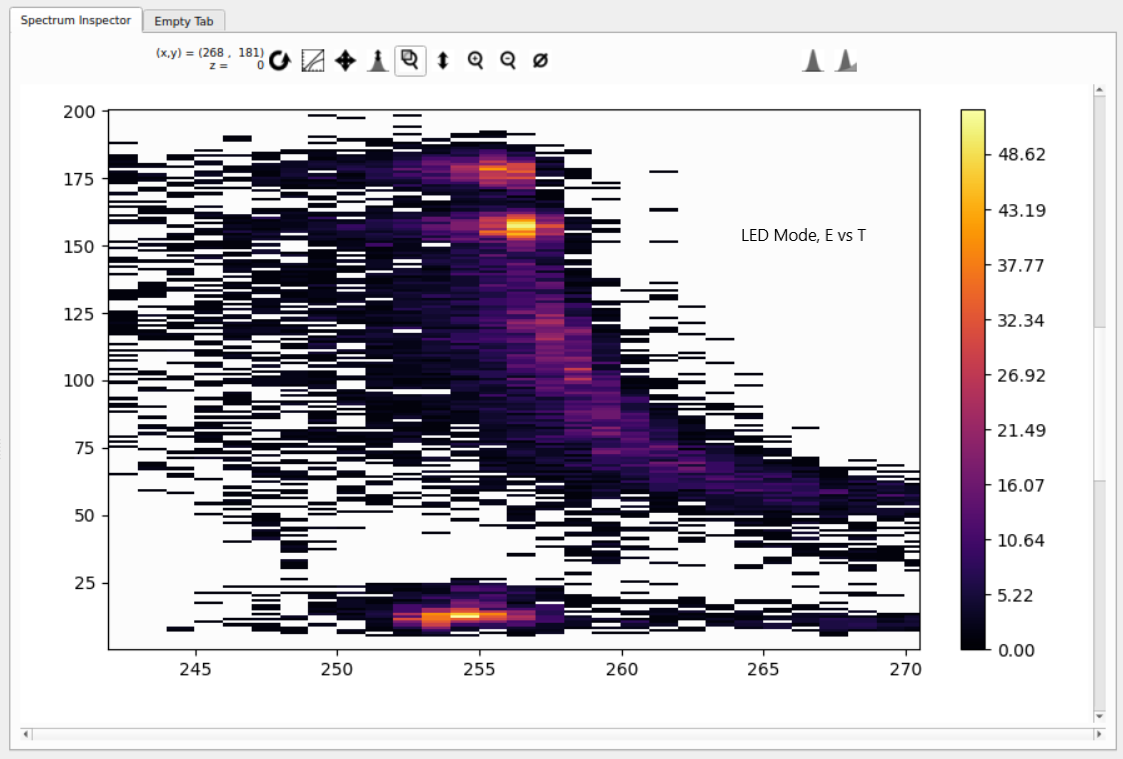
\includegraphics[width=6.5in]{Chapter-5/figs/Co60_LED_EvsT0.png}
%\caption{\label{fig:Co60_LED_EvsT0}}
%\end{figure}

%\begin{figure}[t]
%\centering
%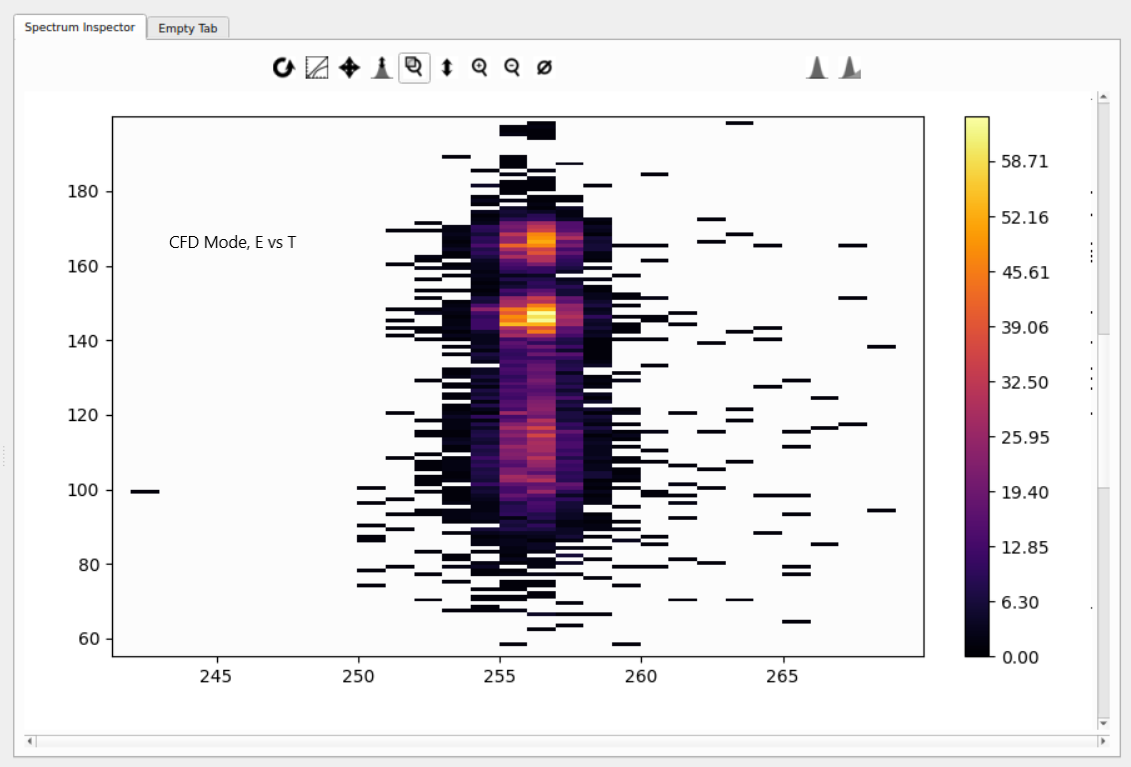
\includegraphics[width=6.5in]{Chapter-5/figs/Co60_CFD_EvsT0.png}
%\caption{\label{fig:Co60_CFD_EvsT0}}
%\end{figure}

\subsection{Development of Coincidence Logic in \texttt{EngeSpec}} \label{subsec:coincidences}

%The timing resolution for the digital DAQ was tested by measuring coincidences. For this purpose, two NaI(Tl) scintillation detectors were needed. 

Acquiring coincidences in the previous section required the use of two detectors, but it also required new developments in the \texttt{EngeSpec} sort routine. The individual $Q_{long}$ and trigger time tag data for each detector needed to be collected and sorted separately. At the time of this test, the software infrastructure for multiple simultaneous channels was not yet developed. The way the CAEN V1730 digitizer couples adjacent channels in its channel aggregate memory structure made this a difficult task. However, this was resolved, and the implementation was rapidly extended to all 16 channels simultaneously. The infrastructure for obtaining coincidences also had to be developed. This is traditionally handled by analog modules, but the \texttt{EngeSpec} sort routine can now handle coincidences entirely on its own. 

There are currently two versions, in terms of coincidence development, of the \texttt{EngeSpec} sort routine. The first attempt was for the above case where 2 and only 2 channels are in coincidence. In this case, coincidence candidates must occur consecutively between the 2 channels. In other words, a flag is raised if two events from the same channel are collected consecutively. Furthermore, they must have a sufficiently small timetag difference such that they fit in the coincidence histogram, with the range specified by the user. This is not very sophisticated, but it clearly served the purpose for the timing resolution test, as this was the version that was used. 

The second version came later, where coincidence logic was developed with the focal plane detector electronics in mind. In this updated case, a coincidence window is opened when an event is collected from the specified triggering channel, where the total time for the window is user-defined. Coincidences are achieved only if an event from a different channel is collected within that window. The relative times are kept track of with the trigger time tag data for each event.

%\subsection{Coincidences with NaI Detectors}

%\subsubsection{LED Mode}

%\paragraph{Timing Spectrum}

%\paragraph{2D Energy Spectrum}

%\paragraph{2D Energy vs. Coincidence Time Spectrum}

%\paragraph{Gating on Timing Spectrum}

%\subsubsection{CFD Mode}

%\paragraph{Timing Spectrum}

%\paragraph{2D Energy Spectrum}

%\paragraph{2D Energy vs. Coincidence Time Spectrum}

%\subsection{Dead Time Tests with Fixed Energy Pulser}

\section{Conclusions}

A digital data acquisition system has been developed at the Triangle Universities Nuclear Laboratory that will replace the traditional analog module system for the focal plane detector package used with the Enge Split-Pole Spectrograph. The CAEN V1730 digitizer is the main component of the new system. Its digital pulse processing algorithms emulate the effects of analog modules, and frontend software has been developed to write user-defined settings to their associated registry addresses on the digitizer board. A settings file is read by the frontend software for ease of access to the registries. A system in which extraction and sorting of the important quantities associated with each detector event, such as its energy and time tag, has also been developed.

Initial tests were performed on the resolution of these quantities using radioisotopes with NaI(Tl) detectors. An energy resolution of 5.5$\%$ has been determined with a $^{152}$Eu source when the long gate parameter responsible for charge integration is optimized. A timing resolution of 4.75 ns (FWHM) has also been determined through coincidence studies with a $^{60}$Co source and two NaI(Tl) detectors when constant fraction discrimination is enabled over leading edge discrimination. As a result of the timing resolution test, significant progress was made in the development of coincidence logic in the sort routine of the graphical user interface \texttt{EngeSpec}. A sort routine appropriate for signals from the focal plane detector package at the Enge Split-Pole Spectrograph has been developed as a result, which handles coincidence and triggering logic. This system will soon be commissioned at TUNL.